%=====================================================================
%  News Topic Classification on AG News
%  Sequential and Transformer models implemented from scratch
%  Build:  pdflatex report  (x3, for TOC/refs)  -- see build.sh
%=====================================================================
\documentclass[11pt,a4paper,oneside]{report}

\usepackage{amsmath,amssymb,amsfonts}
\usepackage{graphicx}
\usepackage{longtable}
\usepackage{url,verbatim,color,calc,ifthen,alltt}
\usepackage[hidelinks]{hyperref}

% ---- page geometry (set by hand; the geometry package is unavailable) -------
\setlength{\oddsidemargin}{0.10in}
\setlength{\evensidemargin}{0.10in}
\setlength{\textwidth}{6.20in}
\setlength{\topmargin}{-0.30in}
\setlength{\headheight}{14pt}
\setlength{\headsep}{20pt}
\setlength{\textheight}{9.15in}
\setlength{\parskip}{4pt}
\setlength{\parindent}{0pt}

% ---- booktabs-style rules (the booktabs package is unavailable) -------------
\newcommand{\toprule}{\hline}
\newcommand{\midrule}{\hline}
\newcommand{\bottomrule}{\hline}
\renewcommand{\arraystretch}{1.25}

% ---- colours used in tables/notes ------------------------------------------
\definecolor{accent}{rgb}{0.165,0.471,0.839}
\definecolor{warm}{rgb}{0.922,0.408,0.204}
\definecolor{greyink}{rgb}{0.32,0.32,0.30}

% ---- helpers ---------------------------------------------------------------
\newcommand{\code}[1]{\texttt{\small #1}}
\newcommand{\bs}{\char`\\}
\newcommand{\us}{\char`\_}
% The TS1 text-symbol fonts are not installed in this TeX distribution, so the
% default \textbullet item label is unavailable. Use the math bullet instead.
\renewcommand{\labelitemi}{$\bullet$}
\renewcommand{\labelitemii}{$\circ$}
\newcommand{\paperterm}[1]{\textit{#1}}
\newcommand{\keypoint}[1]{\par\vspace{3pt}\noindent\textbf{#1}}

\hyphenation{Trans-for-mer BiL-STM clas-si-fi-ca-tion}

\begin{document}

%=====================================================================
\begin{titlepage}
\centering
\vspace*{0.6in}

{\Large\bfseries A Comparative Study of Recurrent and\\[6pt]
Self-Attentive Architectures for\\[6pt]
News Topic Classification}\\[10pt]

{\large Sequential and Transformer models implemented from first principles\\
and evaluated on the AG News corpus}\\[0.5in]

\rule{\textwidth}{0.8pt}\\[0.25in]

{\large\textbf{Case Study Report}}\\[6pt]
{\large Transformer Modeling and Sequence Learning}\\[6pt]
{\large Topic 2 --- News Topic Classification Using Sequential and Transformer Models}\\[0.3in]

\rule{\textwidth}{0.8pt}\\[0.5in]

\begin{tabular}{rl}
\textbf{Research question} & How do recurrent networks and Transformers compare\\
                           & at classifying short news texts?\\[8pt]
\textbf{Dataset}           & AG News --- 120{,}000 training / 7{,}600 test articles\\
                           & four classes: World, Sports, Business, Sci/Tech\\[8pt]
\textbf{Models}            & Bidirectional LSTM (hand-written cell and recurrence)\\
                           & Transformer encoder (hand-written self-attention)\\[8pt]
\textbf{Headline result}   & 91.14\% vs 91.05\% test accuracy;\\
                           & difference not statistically significant ($p = 0.754$)\\
\end{tabular}

\vfill
{\large Source code and executed notebook:}\\[4pt]
\url{https://github.com/Ashwin-3cS/transformer-t1}\\[0.3in]
{\large \today}
\end{titlepage}

%=====================================================================
\pagenumbering{roman}
\setcounter{page}{2}

\chapter*{Abstract}
\addcontentsline{toc}{chapter}{Abstract}

This report presents a controlled empirical comparison of two families of sequence model on the
task of four-class news topic classification. A bidirectional Long Short-Term Memory network and a
Transformer encoder are implemented from first principles --- the LSTM gating equations, the
unrolled recurrence, scaled dot-product attention, multi-head projection, sinusoidal positional
encoding and layer normalisation are all written by hand rather than invoked from a deep learning
library --- and are trained and evaluated under an experimental protocol designed so that
architecture is the only free variable.

The study uses the AG News corpus. Following the case-study brief, a stratified subset of 60{,}000
records is drawn from the 120{,}000-document training file and split into 54{,}000 training and
6{,}000 validation examples, while the full official 7{,}600-document test set is held back for a
single final evaluation. Both models consume an identical vocabulary, identical tensors and an
identical training budget, and are matched to within 0.19\% on non-embedding parameter count.

Before any training is performed, nine numerical checks verify the hand-written layers against
reference implementations and against invariants that a correct implementation must satisfy. All
nine pass. This verification step is reported as a substantive part of the methodology rather than
as an implementation detail, because the characteristic failure mode of a hand-written layer is not
a crash but a silently degraded result.

The principal finding is negative and is reported as such. The two architectures achieve 91.14\%
and 91.05\% test accuracy respectively, a difference of 0.09 percentage points. McNemar's exact
test on the paired predictions yields $p = 0.754$, and the models agree on 94.78\% of test
documents, so the difference cannot be distinguished from sampling noise. The two models further
exhibit an identical per-class difficulty ordering and share the same dominant error, confusing
Business with Sci/Tech in approximately 9.4\% of Business documents. The report argues that this
equivalence is a consequence of document length: AG News items have a median of 39 tokens, and
self-attention's structural advantage --- constant path length between distant positions --- has
little to act upon at that scale.

A secondary finding concerns computational cost and runs contrary to the usual expectation. On the
CPU-only hardware used here, and at a sequence length of 64 tokens, the recurrent model trained
1.67 times faster per epoch than the Transformer. The report analyses why, distinguishing the
asymptotic argument for attention --- which concerns parallelisability and growth in sequence
length --- from the constant factors that in fact determine wall-clock time in this regime.

\vspace{8pt}
\noindent\textbf{Keywords:} text classification, recurrent neural networks, long short-term memory,
self-attention, Transformer, AG News, McNemar's test, reproducible machine learning.

%=====================================================================
\tableofcontents
\listoffigures
\listoftables

\clearpage
\pagenumbering{arabic}
\setcounter{page}{1}

%=====================================================================
\chapter{Introduction}
\label{ch:intro}

\section{Background and motivation}

Automatic topic classification of news text is one of the oldest and most durable applications of
natural language processing. News agencies route incoming wire copy to desks; aggregators assemble
sections; recommendation systems filter by interest; archives index by subject. In each case the
underlying computational problem is the same: given a short passage of text, assign it to one of a
small set of editorial categories.

What has changed repeatedly over the past three decades is not the problem but the representation.
Early systems treated a document as an unordered bag of words and applied a linear classifier to
sparse count features. The introduction of distributed word representations replaced sparse
indicators with dense vectors that encoded distributional similarity. Recurrent neural networks
then made it possible to model a document as a \emph{sequence} rather than a set, processing tokens
in order and maintaining a hidden state that in principle summarises everything seen so far. The
Transformer subsequently discarded recurrence altogether, replacing the sequential state with an
attention mechanism that relates every position to every other position directly.

The Transformer's dominance in contemporary NLP is not in dispute. What is less often examined
carefully is \emph{where} its advantage actually comes from, and whether that advantage is present
in every task to which the architecture is applied. The mechanism that makes self-attention
powerful --- a constant-length computational path between any two positions in a sequence --- is
explicitly a statement about \emph{long-range} dependency. It is reasonable to ask what remains of
that advantage when the sequences in question are not long.

This question is not merely academic. A great many deployed text classification systems operate on
short inputs: search queries, product titles, support ticket subjects, headlines. If the
architectural advantage of self-attention is contingent on sequence length, then the
engineering decision for such systems cannot be read off from benchmark leaderboards built on
longer documents.

\section{Problem statement}

The task addressed in this report is four-class topic classification of short news documents. Given
a news item consisting of a headline and a one-sentence description, the system must assign exactly
one of four labels: \emph{World}, \emph{Sports}, \emph{Business}, or \emph{Science/Technology}.

Two properties of this task make it a suitable vehicle for the architectural comparison at hand.

First, the documents are short. In the corpus used here the median document is 39 tokens long. This
places the task squarely in the regime where the long-range-dependency argument for self-attention
is weakest, and therefore where a direct comparison is most informative.

Second, the label set has four classes rather than two. A binary sentiment task yields a single
accuracy number and a largely uninformative confusion structure. Four classes produce a confusion
matrix with twelve off-diagonal cells, which permits a far more detailed account of \emph{how} a
model fails rather than merely how often. As will be shown in Chapter~\ref{ch:results}, the error
structure turns out to be considerably more informative than the headline accuracy.

\section{Research question}

The report addresses a single primary research question:

\begin{quote}
\textbf{How do recurrent networks and Transformers compare at classifying short news texts?}
\end{quote}

This decomposes into four subsidiary questions, each of which is answered empirically:

\begin{enumerate}
\item \textbf{Accuracy.} Does either architecture achieve higher classification accuracy, and is
      any observed difference statistically distinguishable from sampling noise?
\item \textbf{Error structure.} Do the two architectures fail on the same documents and the same
      class boundaries, or do they exhibit different inductive biases?
\item \textbf{Cost.} How do the architectures compare in training time, inference latency and
      parameter efficiency at matched capacity?
\item \textbf{Explanation.} Whatever differences or equivalences are observed, what property of the
      task accounts for them?
\end{enumerate}

\section{Objectives}

The study was conducted with the following concrete objectives.

\begin{enumerate}
\item To implement a bidirectional LSTM classifier from first principles, writing the gating
      equations, the cell-state recurrence and the bidirectional unrolling explicitly rather than
      invoking a library primitive.
\item To implement a Transformer encoder classifier from first principles, writing scaled
      dot-product attention, multi-head projection and merging, sinusoidal positional encoding,
      layer normalisation and the residual block structure explicitly.
\item To verify both implementations numerically against reference implementations and against
      invariants that any correct implementation must satisfy, \emph{before} drawing any
      experimental conclusion from them.
\item To design a training and evaluation protocol in which architecture is the only free
      variable, holding data, preprocessing, capacity and training budget fixed.
\item To evaluate both models on a held-out test set using metrics appropriate to a balanced
      multi-class problem, including a test of statistical significance on the paired predictions.
\item To analyse the computational cost of both architectures and to interpret the result in terms
      of the structural properties of recurrence and attention.
\end{enumerate}

\section{Scope and delimitations}

It is as important to state what this study does \emph{not} attempt as what it does.

\keypoint{Training from scratch, not transfer learning.} Both models are trained from randomly
initialised embeddings on the task data alone. No pretrained representations are used. This is a
deliberate scoping decision: it isolates the architectural question. A comparison involving a
pretrained Transformer would primarily measure the value of pretraining, which is a different and
already well-established result.

\keypoint{Matched capacity, not maximum performance.} The models are deliberately sized to have
near-identical non-embedding parameter counts. Neither is tuned to its maximum achievable accuracy
on AG News. The objective is a fair comparison, not a leaderboard entry.

\keypoint{A controlled subset, not the full corpus.} Following the case-study brief, 60{,}000 of
the 120{,}000 available training records are used. The consequences of this choice are discussed
in Section~\ref{sec:threats}.

\keypoint{One corpus, one language, one document length regime.} All conclusions are drawn from
English-language short news text. The report is explicit, particularly in
Chapter~\ref{ch:discussion}, about which findings are expected to generalise and which are
specific to this regime.

\section{Contributions}

This report makes the following contributions.

\begin{enumerate}
\item \textbf{A fully transparent implementation} of both architectures, in which every
      sequence-modelling operation is written explicitly and is available for inspection. Nothing
      of consequence is hidden inside a library call.

\item \textbf{A verification methodology for hand-written layers.} Nine numerical checks are
      specified, motivated and executed, covering equivalence against reference implementations,
      mathematical invariants, masking correctness and gradient viability. The report argues that
      such verification is not optional for from-scratch work, because the characteristic failure
      mode is silent degradation rather than an observable error.

\item \textbf{A genuinely controlled comparison}, in which data, preprocessing, capacity and
      training budget are held fixed and only the architecture varies.

\item \textbf{A statistically disciplined negative result.} The observed accuracy difference is
      0.09 percentage points. Rather than reporting a winner, the study applies McNemar's exact
      test, finds $p = 0.754$, and concludes that the architectures are indistinguishable on this
      task. The report treats the significance test as essential rather than decorative.

\item \textbf{A cost finding that contradicts the expected result}, together with an analysis that
      distinguishes the asymptotic argument for attention from the constant factors that determine
      wall-clock time at short sequence lengths.
\end{enumerate}

\section{Organisation of this report}

The remainder of the report is structured as follows.

\textbf{Chapter~\ref{ch:literature}} reviews the development of text classification from sparse
feature methods through recurrent architectures to self-attention, and surveys published results
on the AG News benchmark in order to situate the present work.

\textbf{Chapter~\ref{ch:theory}} develops the mathematical background: the recurrent formulation
and its gradient pathology, the LSTM gating solution, the attention mechanism and its scaling, and
a complexity analysis that formalises the structural trade-off between the two architectures.

\textbf{Chapter~\ref{ch:method}} describes the corpus, the data cleaning required, the controlled
experimental design, the preprocessing pipeline and the evaluation metrics.

\textbf{Chapter~\ref{ch:implementation}} presents the implementation of both models, with
attention to the specific points at which a from-scratch implementation is most likely to go
wrong.

\textbf{Chapter~\ref{ch:verification}} presents the nine verification checks, their motivation and
their results.

\textbf{Chapter~\ref{ch:results}} reports the experimental results: training dynamics, accuracy,
per-class performance, confusion structure, statistical significance, computational cost and a
qualitative error analysis.

\textbf{Chapter~\ref{ch:discussion}} interprets the results, answers the research question,
compares the findings with published work, and states the threats to validity.

\textbf{Chapter~\ref{ch:conclusion}} concludes and identifies future work.

The appendices contain the full source listings of the hand-written components, the complete
classification reports, and instructions for reproducing every number in this document.

\chapter{Literature Review}
\label{ch:literature}

\section{Overview}

This chapter traces the development of neural text classification in order to establish where the
present comparison sits. The narrative is organised around a single recurring question: \emph{how
is word order represented?} Each major advance in the field can be read as a different answer to
that question, and the two architectures compared in this report represent the two most recent
answers.

\section{The sparse feature era}

The earliest statistical approaches to text classification represented a document as a vector of
term counts or weighted term frequencies, discarding word order entirely. The bag-of-words model,
typically weighted by term frequency--inverse document frequency (TF--IDF), paired with a linear
classifier such as multinomial Naive Bayes or a support vector machine, formed the standard
baseline for many years \cite{joachims1998}.

These methods remain surprisingly competitive on topic classification specifically. Topic is
largely signalled by lexical choice: the presence of the words \emph{quarterly}, \emph{earnings}
and \emph{shares} is close to sufficient evidence for a business story, irrespective of the order
in which those words appear. This observation matters for the present study, because it implies
that topic classification is a task where sequential modelling has comparatively little to
contribute --- a point returned to in Chapter~\ref{ch:discussion}.

The principal weaknesses of the sparse approach are the dimensionality of the feature space, the
absence of any notion of semantic similarity between distinct terms, and the inability to
represent negation, modification or any other order-dependent phenomenon.

\section{Distributed word representations}

The second weakness was addressed by distributed representations. Word2Vec \cite{mikolov2013}
and GloVe \cite{pennington2014} learn dense, low-dimensional vectors such that distributionally
similar words occupy nearby regions of the space. A document can then be represented by, for
example, the mean of its word vectors --- a representation that generalises across synonyms in a
way that sparse indicators cannot.

Word order, however, remains unmodelled. Averaging word vectors is still a bag-of-words
operation. The FastText classifier \cite{joulin2017} demonstrated that this simple approach,
with the addition of character n-gram features, achieves strong results on topic classification at
a tiny fraction of the computational cost of neural sequence models --- again suggesting that the
marginal value of sequence modelling on this class of task is modest.

\section{Recurrent neural networks}

Recurrent neural networks introduced genuine sequential modelling. An RNN maintains a hidden state
$h_t$ that is updated at each timestep as a function of the current input and the previous state,
so that in principle $h_T$ summarises the entire sequence.

In practice, the simple recurrent formulation suffers from the vanishing and exploding gradient
problem, analysed by Bengio et al.\ \cite{bengio1994} and later in detail by Pascanu et al.\
\cite{pascanu2013}. Because backpropagation through time multiplies Jacobian matrices once per
timestep, gradient magnitude decays or grows geometrically with the distance over which credit
must be assigned. The practical consequence is that simple RNNs fail to learn dependencies
spanning more than a handful of timesteps. The formal statement of this result is developed in
Section~\ref{sec:vanishing}.

\section{Long Short-Term Memory}

The Long Short-Term Memory architecture of Hochreiter and Schmidhuber \cite{hochreiter1997}
addresses the gradient pathology directly. LSTM introduces a separate \emph{cell state} that is
modified by additive rather than multiplicative interactions, and three multiplicative gates ---
input, forget and output --- that control the flow of information into, within and out of the
cell. Gers et al.\ \cite{gers2000} subsequently added the forget gate in the form now considered
standard.

The critical structural property is that the cell state path from $c_{t-1}$ to $c_t$ passes through
an addition and an elementwise multiplication by the forget gate, rather than through a weight
matrix and a saturating nonlinearity. When the forget gate is near one, gradients propagate
backwards along this path essentially unattenuated. This is the mechanism by which LSTM extends
the effective credit-assignment horizon from a handful of timesteps to hundreds.

The Gated Recurrent Unit \cite{cho2014} simplifies the LSTM to two gates and a single state
vector, with broadly comparable empirical performance and fewer parameters. The present study uses
LSTM rather than GRU because its gate structure is the canonical formulation and its correspondence
with the reference implementation used for verification (Chapter~\ref{ch:verification}) is exact.

\section{Bidirectionality}

A unidirectional recurrent network computes a representation of each position conditioned only on
the preceding context. For classification --- where the entire document is available at inference
time and there is no requirement to generate left to right --- this is an unnecessary restriction.
Bidirectional recurrent networks \cite{schuster1997} run two independent recurrences, one in each
direction, and concatenate the resulting representations, so that each position is contextualised
by both its left and right neighbourhoods.

Bidirectionality is standard in recurrent text classification and is used in the present study.
Note that it doubles the sequential computation, which is relevant to the cost analysis in
Chapter~\ref{ch:results}.

\section{Attention}

Attention was introduced by Bahdanau et al.\ \cite{bahdanau2015} in the context of neural machine
translation, as a mechanism to relieve the bottleneck of compressing an entire source sentence
into a single fixed-length vector. Rather than conditioning on a single summary state, the decoder
computes a weighted combination of all encoder states, with weights determined by a learned
compatibility function between the decoder's current state and each encoder position.

Luong et al.\ \cite{luong2015} simplified the compatibility function to a dot product and
systematised the variants. The essential insight --- that a model can learn \emph{where to look}
rather than being forced to summarise everything into one vector --- proved far more general than
its original application.

\section{The Transformer}

Vaswani et al.\ \cite{vaswani2017} took the decisive step of removing recurrence entirely. The
Transformer computes representations using \emph{self}-attention, in which every position attends
to every other position in the same sequence, combined with position-wise feed-forward layers,
residual connections and layer normalisation \cite{ba2016}.

Two properties of this design are central to the argument of this report.

\keypoint{Constant path length.} In a recurrent network, information must traverse $O(n)$
sequential steps to travel between positions $n$ apart. In self-attention, every pair of positions
is connected directly, so the path length is $O(1)$. This is the structural basis of the
Transformer's advantage on long-range dependency.

\keypoint{Parallelism.} Recurrence is inherently sequential: step $t$ cannot be computed until step
$t-1$ is complete. Self-attention has no such constraint; all positions are computed
simultaneously as a batched matrix product. On parallel hardware this translates directly into
reduced wall-clock time per training step.

Because self-attention is permutation-invariant, positional information must be injected
explicitly. The original work uses fixed sinusoidal encodings; learned positional embeddings are a
common alternative. The pre-norm variant of the residual block, in which layer normalisation is
applied before rather than after each sublayer, was shown by Xiong et al.\ \cite{xiong2020} to
yield better-conditioned gradients at initialisation and to remove the need for a learning-rate
warmup schedule. The present study uses the pre-norm arrangement for precisely this reason.

\section{Pretrained language models}

BERT \cite{devlin2019} demonstrated that a Transformer encoder pretrained on a large unlabelled
corpus with a masked language modelling objective, then fine-tuned on a downstream task,
substantially outperforms task-specific architectures trained from scratch. The paradigm now
dominates the field, with RoBERTa \cite{liu2019} and numerous successors refining the recipe.

It is important to be precise about what this result establishes. The gain attributable to BERT on
a task such as AG News comes overwhelmingly from \emph{pretraining} --- from representations
learned on billions of words of unlabelled text --- rather than from self-attention as an
architectural primitive. Conflating the two is a common error, and the present study is explicitly
designed to avoid it: by training both architectures from scratch on identical data, the
comparison isolates the architectural contribution.

\section{Large language models and the current landscape}

The most recent development is the application of large generative language models to
classification, either zero-shot, few-shot, or via instruction tuning. A 2024 study on text
classification in the age of large language models \cite{mdpi2024} --- identified in the
case-study brief as the related work for this topic --- examines this landscape and reports a
finding directly relevant here: for well-specified classification tasks with adequate labelled
data, compact supervised models remain competitive with, and far cheaper than, large generative
models. The persistent value of small task-specific classifiers is a recurring conclusion in this
literature, and it motivates continued careful study of exactly the architectures compared in this
report.

\section{Prior results on AG News}

AG News was introduced as a classification benchmark by Zhang et al.\ \cite{zhang2015}, who used
it to evaluate character-level convolutional networks. It has since become a standard
four-class topic classification benchmark. Table~\ref{tab:prior} summarises representative
published accuracies.

\begin{table}[ht]
\centering
\caption[Representative published results on AG News]{Representative published test accuracies on
the AG News benchmark. Figures are as reported in the cited work and are not strictly comparable,
since training budgets, preprocessing and the use of pretraining differ. They are presented to
situate the present study rather than to rank methods.}
\label{tab:prior}
\begin{tabular}{lll}
\toprule
\textbf{Approach} & \textbf{Family} & \textbf{Reported accuracy} \\
\midrule
Bag of words + linear classifier \cite{zhang2015}   & Sparse features   & $\approx 88.8\%$ \\
FastText \cite{joulin2017}                          & Embedding average & $\approx 92.5\%$ \\
Character-level CNN \cite{zhang2015}                & Convolutional     & $\approx 90.5\%$ \\
Word-level CNN / LSTM baselines \cite{zhang2015}    & Neural sequence   & $\approx 90$--$92\%$ \\
BERT-base fine-tuned \cite{devlin2019,liu2019}      & Pretrained Transformer & $\approx 94$--$95\%$ \\
\bottomrule
\end{tabular}
\end{table}

Three observations follow from this table and are important context for the results reported later.

First, the spread between a simple bag-of-words classifier and a fine-tuned BERT model is roughly
six percentage points. This is a comparatively narrow band, and it indicates that AG News is a
task on which lexical evidence carries most of the signal.

Second, the models in the middle of this range --- FastText, character CNNs, word-level recurrent
and convolutional baselines --- are clustered tightly around 90--92\%. Architectures of very
different character arrive at very similar accuracy, which is itself suggestive.

Third, the models at the top of the range are distinguished by pretraining, not by architecture.
The present study, which trains from scratch, should therefore be expected to land in the 90--92\%
band, and does.

\section{Research gap}

The literature establishes that Transformers outperform recurrent networks on a wide range of
tasks, and that pretrained Transformers outperform everything. What is less well documented is a
careful, controlled comparison of the two architectures \emph{at matched capacity}, \emph{without
pretraining}, on \emph{short} text, with \emph{statistical testing} of the resulting difference.

Published comparisons frequently differ in parameter count, training budget, preprocessing or
tokenisation between the systems being compared, which makes the attribution of any observed
difference to architecture unsafe. Significance testing of classification differences is uncommon,
despite accuracy differences of under one percentage point being routinely reported as
improvements.

This report addresses that gap for one specific and practically important regime: short-text topic
classification. It holds data, preprocessing, capacity and training budget fixed; it verifies both
implementations numerically before drawing conclusions from them; and it applies a paired
significance test to the resulting predictions.

\chapter{Theoretical Background}
\label{ch:theory}

This chapter develops the mathematics of the two architectures. The treatment is deliberately
explicit, because the implementations in Chapter~\ref{ch:implementation} follow these equations
term by term, and the verification in Chapter~\ref{ch:verification} checks them numerically.

\section{Problem formalisation}

Let $\mathcal{V}$ be a finite vocabulary and let a document be a sequence of tokens
$x = (x_1, x_2, \dots, x_n)$ with $x_t \in \mathcal{V}$. Let $\mathcal{C} = \{1, \dots, K\}$ be a
set of $K$ class labels; here $K = 4$.

The task is to learn a function $f_\theta : \mathcal{V}^{*} \rightarrow \Delta^{K-1}$, mapping a
token sequence of arbitrary length to a probability distribution over the $K$ classes, where
$\Delta^{K-1}$ denotes the probability simplex. Given a labelled training set
$\mathcal{D} = \{(x^{(i)}, y^{(i)})\}_{i=1}^{N}$, the parameters $\theta$ are chosen to minimise
the categorical cross-entropy
\begin{equation}
\mathcal{L}(\theta) = -\frac{1}{N} \sum_{i=1}^{N} \log f_\theta(x^{(i)})_{y^{(i)}} .
\label{eq:xent}
\end{equation}

Both architectures studied here share a common three-stage structure:
\begin{enumerate}
\item an \textbf{embedding} stage mapping tokens to dense vectors,
\item a \textbf{contextualisation} stage producing position-wise representations that depend on the
      rest of the sequence --- this is the stage in which the two architectures differ,
\item a \textbf{pooling and classification} stage reducing the variable-length sequence of
      representations to a single vector and projecting it to $K$ logits.
\end{enumerate}

Holding stages 1 and 3 as similar as possible while varying stage 2 is precisely the experimental
design described in Chapter~\ref{ch:method}.

\section{Embedding}

An embedding matrix $E \in \mathbb{R}^{|\mathcal{V}| \times d}$ maps each token index to a row
vector. For a sequence $x$ of length $n$ this yields
\begin{equation}
X = \big(E_{x_1}, E_{x_2}, \dots, E_{x_n}\big)^{\!\top} \in \mathbb{R}^{n \times d}.
\end{equation}
In this study $E$ is randomly initialised and learned jointly with the rest of the model; no
pretrained vectors are used. A designated padding index is held at the zero vector and excluded
from gradient updates.

\section{Recurrent networks and the vanishing gradient problem}
\label{sec:vanishing}

\subsection{The simple recurrent formulation}

A simple recurrent network maintains a hidden state updated at each timestep:
\begin{equation}
h_t = \phi\big(W x_t + U h_{t-1} + b\big), \qquad h_0 = \mathbf{0},
\label{eq:rnn}
\end{equation}
where $\phi$ is a saturating nonlinearity, typically $\tanh$.

\subsection{Backpropagation through time}

Training requires the gradient of a loss $\mathcal{L}$ defined at the final timestep with respect
to parameters that are shared across all timesteps. Applying the chain rule across the unrolled
computation gives
\begin{equation}
\frac{\partial \mathcal{L}}{\partial h_k}
  = \frac{\partial \mathcal{L}}{\partial h_n}
    \prod_{t=k+1}^{n} \frac{\partial h_t}{\partial h_{t-1}} .
\label{eq:bptt}
\end{equation}
From Equation~\ref{eq:rnn}, each Jacobian factor is
\begin{equation}
\frac{\partial h_t}{\partial h_{t-1}}
  = U^{\!\top} \operatorname{diag}\!\big(\phi'(a_t)\big),
  \qquad a_t = W x_t + U h_{t-1} + b .
\end{equation}

\subsection{The pathology}

Taking norms in Equation~\ref{eq:bptt} and writing $\gamma = \sup_z |\phi'(z)|$ --- which equals
$1$ for $\tanh$ and $\tfrac{1}{4}$ for the logistic sigmoid --- gives the bound
\begin{equation}
\left\| \frac{\partial h_t}{\partial h_{t-1}} \right\| \;\le\; \gamma \, \|U\| ,
\qquad\text{hence}\qquad
\left\| \prod_{t=k+1}^{n} \frac{\partial h_t}{\partial h_{t-1}} \right\|
  \;\le\; \big(\gamma \|U\|\big)^{\,n-k} .
\label{eq:vanish}
\end{equation}

The product is geometric in the distance $n-k$. If $\gamma\|U\| < 1$ the gradient decays
exponentially and the network cannot assign credit across long spans --- the \emph{vanishing
gradient} problem. If $\gamma\|U\| > 1$ it grows exponentially --- the \emph{exploding gradient}
problem, which is the more tractable of the two and is routinely handled by gradient-norm
clipping, as is done in this study.

Vanishing gradients cannot be addressed by clipping, because the information is destroyed rather
than merely rescaled. The resolution requires an architectural change.

\section{Long Short-Term Memory}

\subsection{Gating equations}

LSTM introduces a cell state $c_t$ alongside the hidden state $h_t$, together with three gates. At
each timestep:
\begin{align}
i_t &= \sigma\!\left(W_i x_t + U_i h_{t-1} + b_i\right) && \text{input gate} \label{eq:lstm_i}\\
f_t &= \sigma\!\left(W_f x_t + U_f h_{t-1} + b_f\right) && \text{forget gate} \label{eq:lstm_f}\\
g_t &= \tanh\!\left(W_g x_t + U_g h_{t-1} + b_g\right) && \text{candidate cell} \label{eq:lstm_g}\\
o_t &= \sigma\!\left(W_o x_t + U_o h_{t-1} + b_o\right) && \text{output gate} \label{eq:lstm_o}\\
c_t &= f_t \odot c_{t-1} + i_t \odot g_t && \text{cell update} \label{eq:lstm_c}\\
h_t &= o_t \odot \tanh(c_t) && \text{hidden output} \label{eq:lstm_h}
\end{align}
where $\sigma$ is the logistic sigmoid and $\odot$ denotes elementwise multiplication.

Interpretively: the forget gate $f_t$ decides what proportion of the existing cell contents to
retain; the input gate $i_t$ decides how much of the new candidate $g_t$ to admit; and the output
gate $o_t$ decides how much of the resulting cell state to expose as the hidden output.

\subsection{Why this solves the gradient problem}

Consider the derivative of the cell state with respect to its own previous value. Differentiating
Equation~\ref{eq:lstm_c}, and noting that $f_t$, $i_t$ and $g_t$ all depend on $h_{t-1}$ rather
than on $c_{t-1}$ directly, the dominant term is
\begin{equation}
\frac{\partial c_t}{\partial c_{t-1}} \;=\; \operatorname{diag}(f_t) \;+\; (\text{terms via } h_{t-1}).
\label{eq:lstm_grad}
\end{equation}

The leading term is multiplication by the forget gate, with \emph{no weight matrix and no
saturating nonlinearity in the path}. When $f_t \approx \mathbf{1}$, the gradient flows backwards
across that timestep essentially unchanged. Over $n-k$ steps the decay is governed by
$\prod_t f_t$ rather than by $(\gamma\|U\|)^{n-k}$, and since the forget gate is learned, the
network can \emph{choose} to keep this path open for exactly those features requiring long-range
credit assignment. This is the constant error carousel of the original formulation
\cite{hochreiter1997}, and it is the entire reason LSTM works.

\subsection{Fused gate computation}

Equations~\ref{eq:lstm_i}--\ref{eq:lstm_o} share the same two inputs, $x_t$ and $h_{t-1}$. In
implementation the four gate pre-activations are therefore computed in a single pair of matrix
products,
\begin{equation}
\begin{bmatrix} a_i \\ a_f \\ a_g \\ a_o \end{bmatrix}
  = \underbrace{W x_t}_{\in \mathbb{R}^{4d_h}} + \underbrace{U h_{t-1}}_{\in \mathbb{R}^{4d_h}} + b,
\end{equation}
with $W \in \mathbb{R}^{4d_h \times d}$ and $U \in \mathbb{R}^{4d_h \times d_h}$, after which the
result is split into four equal blocks. This is a pure efficiency transformation --- it is
mathematically identical to the separate form --- but it is the form used in the implementation,
and the \emph{ordering} of the four blocks is a convention that must match the reference
implementation for the verification in Chapter~\ref{ch:verification} to be meaningful.

\subsection{Parameter count}

An LSTM layer with input dimension $d$ and hidden dimension $d_h$ has
\begin{equation}
P_{\text{LSTM}} = 4\big(d\,d_h + d_h^2 + d_h\big)
\end{equation}
parameters. A bidirectional layer doubles this.

\section{Bidirectional recurrence}

A bidirectional layer runs two independent recurrences,
\begin{equation}
\overrightarrow{h}_t = \text{LSTM}^{\rightarrow}(x_t, \overrightarrow{h}_{t-1}), \qquad
\overleftarrow{h}_t  = \text{LSTM}^{\leftarrow}(x_t, \overleftarrow{h}_{t+1}),
\end{equation}
and concatenates them, $h_t = [\overrightarrow{h}_t ; \overleftarrow{h}_t] \in \mathbb{R}^{2d_h}$.
Each position is thereby contextualised by the whole sequence rather than only its prefix.

\section{Pooling}
\label{sec:pooling}

Classification requires reducing $(h_1,\dots,h_n)$ to a single vector. Three strategies are
standard.

\keypoint{Last state.} Use $h_n$. For a unidirectional recurrent model this is the natural
summary, but it is sensitive to the final token and discards earlier evidence except insofar as the
state retained it.

\keypoint{Mean pooling.} Use $\frac{1}{n}\sum_t h_t$. This weights all positions equally and is
robust, but for a recurrent model it discards the privileged endpoint that the recurrence was
constructed to produce.

\keypoint{Concatenation.} Use $\big[\tfrac{1}{n}\sum_t h_t \,;\, \overrightarrow{h}_n \,;\,
\overleftarrow{h}_1\big]$, combining both. This is the strategy adopted here, on the reasoning that
the two summaries carry complementary information and documents of 39 tokens are short enough that
the endpoint alone is noisy.

With padded batches, all pooling operations must be masked --- a point of considerable practical
importance developed in Section~\ref{sec:masking}.

\section{Attention}

\subsection{Scaled dot-product attention}

Given queries $Q \in \mathbb{R}^{n \times d_k}$, keys $K \in \mathbb{R}^{m \times d_k}$ and values
$V \in \mathbb{R}^{m \times d_v}$, scaled dot-product attention is
\begin{equation}
\operatorname{Attention}(Q,K,V)
  = \operatorname{softmax}\!\left(\frac{QK^{\top}}{\sqrt{d_k}}\right) V .
\label{eq:attention}
\end{equation}

The matrix $QK^{\top} \in \mathbb{R}^{n\times m}$ contains a compatibility score for every
query--key pair. The row-wise softmax converts each row into a probability distribution over the
$m$ positions, and the product with $V$ forms, for each query, a convex combination of value
vectors.

In \emph{self}-attention, $Q$, $K$ and $V$ are all linear projections of the same input sequence,
so $n = m$ and every position attends to every position including itself.

\subsection{Why the $\sqrt{d_k}$ scaling is necessary}

The scaling factor is not cosmetic. Suppose the components of $q$ and $k$ are independent with zero
mean and unit variance. Then
\begin{equation}
\operatorname{E}\!\left[q \cdot k\right] = 0,
\qquad
\operatorname{Var}\!\left[q \cdot k\right]
  = \operatorname{Var}\!\left[\sum_{j=1}^{d_k} q_j k_j\right] = d_k .
\end{equation}

The dot products therefore have standard deviation $\sqrt{d_k}$, growing with the head dimension.
For large $d_k$ the softmax receives inputs of large magnitude and saturates: its output approaches
a one-hot vector, and its Jacobian approaches zero. Writing $p = \operatorname{softmax}(s)$, the
Jacobian is
\begin{equation}
\frac{\partial p_i}{\partial s_j} = p_i\big(\delta_{ij} - p_j\big),
\end{equation}
which vanishes as any $p_i \to 1$. Dividing by $\sqrt{d_k}$ restores unit variance to the scores
and keeps the softmax in its responsive region, preserving gradient flow.

\subsection{Multi-head attention}

A single attention operation produces one weighted average per position, which constrains the model
to one relational pattern per layer. Multi-head attention runs $h$ attention operations in
parallel on different learned projections:
\begin{align}
\operatorname{head}_j &= \operatorname{Attention}\!\left(XW_j^{Q},\, XW_j^{K},\, XW_j^{V}\right), \\
\operatorname{MHA}(X) &= \left[\operatorname{head}_1 ; \dots ; \operatorname{head}_h\right] W^{O} .
\label{eq:mha}
\end{align}
With $d_k = d_v = d_{\text{model}}/h$, total computation is approximately that of a single head at
full dimension, but the model can attend to several distinct relational patterns simultaneously.

In implementation the per-head projections are not separate matrices. A single projection of width
$d_{\text{model}}$ is computed and then \emph{reshaped} into $h$ blocks of width $d_k$. This
reshape is the single most error-prone step in implementing attention, and it is the specific
target of verification check~3 in Chapter~\ref{ch:verification}.

\subsection{Masking}
\label{sec:masking}

Batched processing requires padding sequences to a common length. Padded positions must not
influence the result. In attention this is enforced by adding a mask to the scores before the
softmax:
\begin{equation}
s'_{ij} = \begin{cases}
s_{ij} & \text{if position } j \text{ is a real token} \\
-\infty & \text{if position } j \text{ is padding,}
\end{cases}
\end{equation}
so that $\operatorname{softmax}(s')$ assigns exactly zero weight to padded keys.

In practice $-\infty$ is replaced by a large finite negative constant. The reason is numerical: if
an entire row were masked, $\operatorname{softmax}$ of a vector of $-\infty$ evaluates to
$0/0 = \text{NaN}$, which propagates through the network and destroys the gradients. A large
finite constant yields a harmless uniform distribution in that degenerate case.

\section{Positional encoding}

Self-attention as defined in Equation~\ref{eq:attention} is permutation-equivariant: permuting the
input rows permutes the output rows identically, with no other change. A model built from
self-attention alone therefore cannot distinguish word order at all --- it would be a bag-of-words
model with a sophisticated weighting scheme.

Position must consequently be injected explicitly. The sinusoidal scheme of
Vaswani et al.\ \cite{vaswani2017} defines
\begin{align}
PE_{(\text{pos},\,2i)}   &= \sin\!\left(\frac{\text{pos}}{10000^{2i/d_{\text{model}}}}\right), \\
PE_{(\text{pos},\,2i+1)} &= \cos\!\left(\frac{\text{pos}}{10000^{2i/d_{\text{model}}}}\right),
\end{align}
and adds $PE$ to the token embeddings. Each dimension is a sinusoid of a different wavelength,
forming a geometric progression from $2\pi$ to $10000\cdot 2\pi$. The scheme has two useful
properties: it requires no parameters, and because $PE_{\text{pos}+k}$ is a fixed linear function
of $PE_{\text{pos}}$ for any fixed offset $k$, relative position is linearly recoverable.

Token embeddings are scaled by $\sqrt{d_{\text{model}}}$ before the positional signal is added, so
that the two contributions are of comparable magnitude at initialisation.

\section{Layer normalisation}

Layer normalisation \cite{ba2016} standardises each position's feature vector independently:
\begin{equation}
\operatorname{LN}(x) = \gamma \odot \frac{x - \mu}{\sqrt{\varsigma^2 + \epsilon}} + \beta,
\qquad
\mu = \frac{1}{d}\sum_{j=1}^{d} x_j,
\qquad
\varsigma^2 = \frac{1}{d}\sum_{j=1}^{d} (x_j - \mu)^2 ,
\end{equation}
with learned $\gamma, \beta \in \mathbb{R}^{d}$ and a small $\epsilon$ for numerical stability.

Unlike batch normalisation, the statistics are computed over the feature dimension of a single
example, so the operation is independent of batch composition and of sequence length. Note that
$\varsigma^2$ is the \emph{biased} variance, normalising by $d$ rather than $d-1$; this detail
matters for the numerical agreement verified in Chapter~\ref{ch:verification}.

\section{Residual connections and block ordering}

Each sublayer is wrapped in a residual connection, which provides an identity path for gradients.
Two orderings are in use:
\begin{align}
\text{post-norm:}\quad & x \leftarrow \operatorname{LN}\!\big(x + \operatorname{Sublayer}(x)\big), \\
\text{pre-norm:}\quad  & x \leftarrow x + \operatorname{Sublayer}\!\big(\operatorname{LN}(x)\big).
\end{align}

In the post-norm arrangement the residual path passes through a normalisation at every layer, and
at initialisation the expected gradient magnitude scales unfavourably with depth, which in practice
necessitates a learning-rate warmup schedule. In the pre-norm arrangement the residual path is
unobstructed from input to output, gradients are better conditioned at initialisation, and warmup
becomes unnecessary \cite{xiong2020}. The present study uses pre-norm, since the training budget
is a small number of epochs and a warmup schedule would consume a meaningful fraction of it.

The complete encoder block is
\begin{align}
x &\leftarrow x + \operatorname{Dropout}\big(\operatorname{MHA}(\operatorname{LN}(x))\big), \\
x &\leftarrow x + \operatorname{Dropout}\big(W_2\,\operatorname{GELU}(W_1 \operatorname{LN}(x))\big).
\end{align}

\section{Complexity analysis}

Table~\ref{tab:complexity} summarises the structural comparison, following the analysis of
Vaswani et al.\ \cite{vaswani2017}. Let $n$ be sequence length and $d$ the representation
dimension.

\begin{table}[ht]
\centering
\caption[Complexity comparison of recurrent and self-attentive layers]{Per-layer complexity,
sequential depth and maximum path length. \emph{Sequential operations} counts steps that cannot be
parallelised; \emph{maximum path length} is the number of computational steps separating the two
most distant positions.}
\label{tab:complexity}
\begin{tabular}{lccc}
\toprule
\textbf{Layer type} & \textbf{Complexity per layer} & \textbf{Sequential operations} & \textbf{Max path length} \\
\midrule
Recurrent (LSTM)    & $O(n \cdot d^2)$ & $O(n)$ & $O(n)$ \\
Self-attention      & $O(n^2 \cdot d)$ & $O(1)$ & $O(1)$ \\
\bottomrule
\end{tabular}
\end{table}

Three consequences follow, and all three are tested empirically in Chapter~\ref{ch:results}.

\keypoint{Path length.} Self-attention connects any two positions in one step; recurrence requires
$O(n)$ steps. This is the basis of the Transformer's advantage on long-range dependency. Its
practical value is proportional to how much long-range structure the task actually contains.

\keypoint{Parallelism.} Recurrence requires $O(n)$ strictly sequential steps; self-attention
requires $O(1)$. On parallel hardware this is a decisive advantage in wall-clock terms.

\keypoint{Arithmetic.} The comparison between $O(n d^2)$ and $O(n^2 d)$ depends on the ratio
$n/d$. Self-attention performs \emph{less} total arithmetic only when $n < d$. With $n = 64$ and
$d = 128$, as in this study, the two are of the same order, and neither dominates. This observation
is central to the cost result reported in Section~\ref{sec:cost}, and it is why that result does
not contradict the theory.

\chapter{Dataset and Methodology}
\label{ch:method}

\section{The AG News corpus}

AG News is a topic classification benchmark derived from the AG corpus of news articles, introduced
in its current form by Zhang et al.\ \cite{zhang2015}. Each record consists of a class index, a
headline and a short description. The four classes are balanced by construction.

\begin{table}[ht]
\centering
\caption{Composition of the AG News corpus as distributed.}
\label{tab:corpus}
\begin{tabular}{lrr}
\toprule
\textbf{Split} & \textbf{Records} & \textbf{Per class} \\
\midrule
Training file & 120{,}000 & 30{,}000 \\
Test file     & 7{,}600   & 1{,}900 \\
\midrule
Total         & 127{,}600 & 31{,}900 \\
\bottomrule
\end{tabular}
\end{table}

The corpus was obtained programmatically through the Kaggle API from the dataset
\code{amananandrai/ag-news-classification-dataset}, so that acquisition is reproducible rather than
dependent on a manual download. The four class indices map to \emph{World}, \emph{Sports},
\emph{Business} and \emph{Science/Technology} respectively.

The text field used throughout is the concatenation of headline and description:
\begin{equation*}
\text{text} = \text{Title} \;+\; \text{``.\,''} \;+\; \text{Description}.
\end{equation*}

\section{Data cleaning}
\label{sec:cleaning}

Inspection of the raw CSV files revealed a systematic artefact inherited from the original scrape.
Escape sequences appear \emph{literally} in the text rather than as the control characters they
denote. A representative record reads:

\begin{quote}
\code{Reuters - Short-sellers, Wall Street's dwindling\bs band of ultra-cynics, are
seeing green again.}
\end{quote}

Here \code{\bs b} is a literal backslash followed by the letter \code{b}, not a
backspace. The phrase should read \emph{``dwindling band of ultra-cynics''}.

This is not a cosmetic problem. Under the tokenisation scheme described in
Section~\ref{sec:tokenisation}, the backslash is discarded as a non-matching character and the
surrounding letters are welded into the single token \code{dwindlingband}. Two genuine, frequent
words are replaced by one spurious type that occurs almost nowhere else in the corpus and is
therefore pruned by the minimum-frequency cutoff, mapping to the unknown token at both training and
test time. The net effect is the silent destruction of lexical evidence in exactly the kind of
content-bearing position that matters most for topic classification.

The cleaning step applies the regular expression \code{\bs\bs[a-z]},
replacing each such sequence with a single space, followed by whitespace normalisation. This is
applied identically to both the training and test files, before any split is taken.

\keypoint{Methodological note.} This artefact is easy to overlook, because a model trained on the
uncleaned data still trains and still reports a plausible accuracy. The discovery came from reading
the raw records directly rather than from any error signal. It is reported here because it is
representative of a general principle in applied machine learning: a substantial fraction of
achievable performance is determined before any model is defined.

\section{Experimental design}

\subsection{The controlled subset}

The case-study brief specifies the use of approximately 60{,}000 records for a controlled
experiment. This was implemented as a stratified sample of exactly 15{,}000 records per class drawn
from the 120{,}000-record training file with a fixed random seed, subsequently shuffled and split
into training and validation partitions.

\begin{table}[ht]
\centering
\caption{Data splits used in the experiment. The test set is the full official file and is used
once, for the final evaluation reported in Chapter~\ref{ch:results}.}
\label{tab:splits}
\begin{tabular}{lrrl}
\toprule
\textbf{Split} & \textbf{Records} & \textbf{Per class} & \textbf{Purpose} \\
\midrule
Training   & 54{,}000 & 13{,}500 & parameter estimation \\
Validation & 6{,}000  & 1{,}500  & early stopping, learning-rate selection \\
Test       & 7{,}600  & 1{,}900  & final evaluation only \\
\bottomrule
\end{tabular}
\end{table}

All three partitions are exactly class-balanced, so accuracy and macro-averaged $F_1$
are directly interpretable and a majority-class baseline sits at 25\%.

\subsection{The four experimental controls}

The comparison is designed so that architecture is the only free variable. Four quantities are held
fixed.

\begin{enumerate}
\item \textbf{Data.} One subset, one split, one fixed seed. Both models see identical records in an
      identical order.

\item \textbf{Preprocessing.} One tokeniser, one vocabulary, one maximum sequence length. The
      integer tensors fed to the two models are not merely equivalent --- they are the same
      objects.

\item \textbf{Capacity.} Both models are sized to approximately 265{,}000 non-embedding
      parameters, a difference of 0.19\%. Without this control, any observed difference could be
      attributed to model size rather than architecture.

\item \textbf{Training budget.} Identical batch size, epoch cap, optimiser family, weight decay,
      gradient clipping, early-stopping criterion and random seed.
\end{enumerate}

\subsection{The one quantity that is not shared}

The learning rate differs between the two models: $10^{-3}$ for the recurrent model and
$3\times10^{-4}$ for the Transformer. Both values were selected on the validation split and never
on the test set.

This choice warrants explicit defence, since it appears to weaken the control. Imposing a single
shared learning rate would \emph{appear} fairer, but it would in fact handicap whichever
architecture that particular value suited less well, and the experiment would then measure
sensitivity to one arbitrary hyperparameter rather than the architectures themselves. Recurrent
and self-attentive models are known to have different stable learning-rate regimes. The quantity
that is properly controlled is the \emph{compute budget}; the learning rate is a per-architecture
tuning decision made on data that is not used for evaluation.

\section{Preprocessing}
\label{sec:tokenisation}

\subsection{Tokenisation}

Documents are lowercased and tokenised with the regular expression
\code{[a-z0-9']+}, which extracts maximal runs of alphanumeric characters and apostrophes. This
retains contractions and possessives as single tokens while discarding punctuation.

The tokeniser is deliberately simple. A more sophisticated scheme --- subword segmentation, for
instance --- would very likely improve both models. It is omitted precisely because both models
must receive identical input: any tokeniser sophistication is a confound if it happens to suit one
architecture better than the other. The simple scheme makes the comparison clean at a small cost in
absolute accuracy.

\subsection{Vocabulary}

The vocabulary is constructed from the \emph{training split only}. Neither the validation nor the
test text contributes any token to the vocabulary, which eliminates a subtle and common form of
information leakage.

Types occurring fewer than twice in the training split are discarded. Two special tokens are
reserved: index $0$ for padding and index $1$ for unknown tokens. The resulting vocabulary contains
\textbf{33{,}964} types.

\subsection{Sequence length}

Choosing a maximum sequence length is a trade-off between truncating information and wasting
computation on padding. The choice was made from the measured distribution rather than by
convention.

\begin{table}[ht]
\centering
\caption{Token-length statistics of the training split.}
\label{tab:lengths}
\begin{tabular}{lr}
\toprule
\textbf{Statistic} & \textbf{Tokens} \\
\midrule
Median                  & 39 \\
Mean                    & 39.4 \\
95th percentile         & 58 \\
Maximum                 & 181 \\
\midrule
Chosen \code{MAX\us{}LEN}  & 64 \\
Coverage at this length & 96.94\% \\
\bottomrule
\end{tabular}
\end{table}

Figure~\ref{fig:lengths} shows the full distribution. A cutoff of 64 tokens leaves 96.94\% of
training documents untruncated while keeping the sequence dimension small enough for the recurrent
model to remain tractable on CPU.

\begin{figure}[ht]
\centering
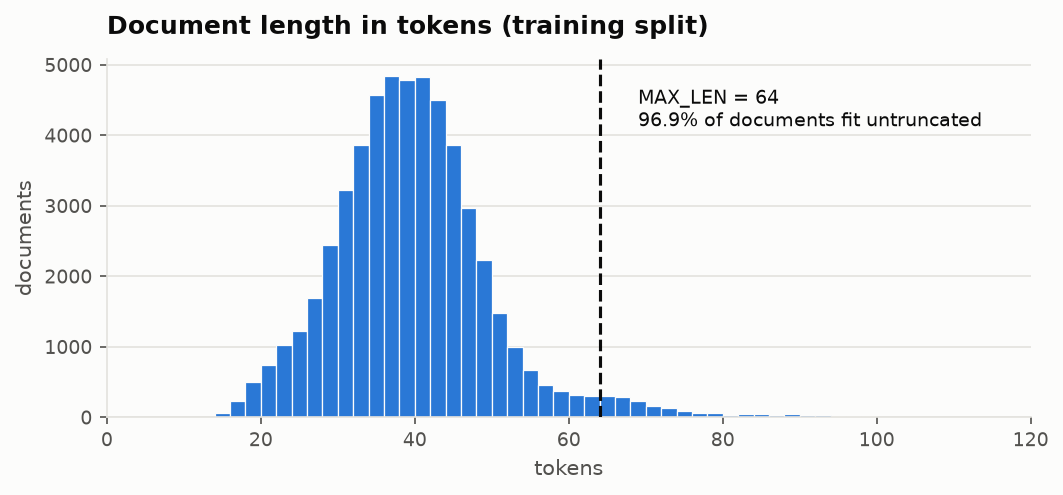
\includegraphics[width=0.92\textwidth]{figures/fig0_token_lengths.png}
\caption[Distribution of document lengths]{Distribution of document lengths in tokens on the
training split. The dashed line marks the chosen cutoff of 64 tokens. The distribution is tightly
concentrated around a median of 39 tokens --- the property that, as argued in
Chapter~\ref{ch:discussion}, accounts for the equivalence of the two architectures.}
\label{fig:lengths}
\end{figure}

\keypoint{The central statistic of this study.} The median document is 39 tokens long. Every
substantive conclusion in Chapter~\ref{ch:discussion} follows from this number.

\subsection{Encoding}

Each document is converted to a fixed-length vector of 64 integer indices, truncated or
right-padded with the padding index as required, together with its true length. Documents reducing
to zero tokens are mapped to a single unknown token so that no sequence has a zero-length mask.

\section{Evaluation metrics}

\subsection{Accuracy and $F_1$}

Since all splits are exactly balanced, accuracy is a meaningful primary metric. It is nonetheless
reported alongside per-class precision, recall and $F_1$:
\begin{equation}
P_c = \frac{TP_c}{TP_c + FP_c}, \qquad
R_c = \frac{TP_c}{TP_c + FN_c}, \qquad
F1_c = \frac{2 P_c R_c}{P_c + R_c}.
\end{equation}

Macro-averaged $F_1$ --- the unweighted mean of the per-class values --- is used as
the model selection criterion, because it weights all four classes equally and is sensitive to
failure on any single class in a way that accuracy is not.

\subsection{Confusion matrix}

The $4\times4$ confusion matrix is reported row-normalised, so that entry $(i,j)$ gives the
proportion of true class $i$ predicted as class $j$. With four classes there are twelve
off-diagonal cells, and their structure is considerably more informative about model behaviour
than any scalar summary.

\subsection{McNemar's test}
\label{sec:mcnemar}

Comparing two classifiers on the same test set produces \emph{paired} observations, and a test
that respects the pairing is required. McNemar's test \cite{mcnemar1947} considers only the
discordant cases --- documents on which the two models disagree --- arranged as:

\begin{table}[ht]
\centering
\caption{Contingency structure for McNemar's test.}
\label{tab:mcnemar_structure}
\begin{tabular}{lcc}
\toprule
 & \textbf{Model B correct} & \textbf{Model B wrong} \\
\midrule
\textbf{Model A correct} & $a$ & $b$ \\
\textbf{Model A wrong}   & $c$ & $d$ \\
\bottomrule
\end{tabular}
\end{table}

The counts $a$ and $d$ --- cases where both models agree --- carry no information about which model
is better and are discarded. Under the null hypothesis that the two models have equal error rates,
each discordant case is equally likely to fall in cell $b$ or cell $c$, so
\begin{equation}
b \sim \operatorname{Binomial}(b + c,\; 0.5).
\end{equation}
The exact binomial test on this statistic is used here in preference to the chi-squared
approximation, since it is valid for any count.

\keypoint{Why this matters.} Accuracy differences below one percentage point are routinely reported
as improvements in the literature. On a 7{,}600-document test set, a difference of 0.09 percentage
points corresponds to seven documents. Without a paired significance test there is no principled
basis for distinguishing such a difference from sampling noise, and as Chapter~\ref{ch:results}
shows, in this case it cannot be so distinguished.

\section{Experimental environment}

\begin{table}[ht]
\centering
\caption{Hardware and software environment. All timing results in Chapter~\ref{ch:results} are
specific to this configuration.}
\label{tab:environment}
\begin{tabular}{ll}
\toprule
\textbf{Component} & \textbf{Specification} \\
\midrule
Processor        & 12 logical cores, 6 PyTorch threads \\
Accelerator      & none --- CPU execution only \\
Memory           & 15\,GB \\
Operating system & Linux (Fedora, kernel 6.17) \\
Python           & 3.14.8 \\
PyTorch          & 2.15.0 (CPU build) \cite{paszke2019} \\
Random seed      & 42, applied to \code{random}, \code{numpy} and \code{torch} \\
\bottomrule
\end{tabular}
\end{table}

The absence of a GPU is not incidental to the findings. It materially affects the cost comparison
in Section~\ref{sec:cost}, and the discussion there is explicit about which conclusions are
hardware-dependent.

\chapter{Implementation}
\label{ch:implementation}

\section{The from-scratch constraint}

Both models are implemented from first principles. The precise meaning of that constraint is
important, and is stated here before the code is presented.

PyTorch is used for three things: multidimensional array arithmetic, reverse-mode automatic
differentiation, and the optimiser. The modules \code{nn.Linear}, \code{nn.Embedding} and
\code{nn.Dropout} are used, but only as containers for learnable parameters --- an
\code{nn.Linear} is an affine map, not a sequence-modelling primitive.

Every operation specific to sequence modelling is written out. Table~\ref{tab:scratch} lists the
correspondence between the theory of Chapter~\ref{ch:theory} and the implementation.

\begin{table}[ht]
\centering
\caption{Components implemented from first principles, with the equations they realise.}
\label{tab:scratch}
\begin{tabular}{lll}
\toprule
\textbf{Component} & \textbf{Implemented as} & \textbf{Equations} \\
\midrule
LSTM gating               & \code{LSTMCellScratch}                & \ref{eq:lstm_i}--\ref{eq:lstm_h} \\
Recurrence, bidirectional & \code{LSTMLayerScratch}               & Sec.~\ref{sec:vanishing} \\
Recurrent classifier      & \code{BiLSTMClassifier}               & Sec.~\ref{sec:pooling} \\
Positional encoding       & \code{sinusoidal\us{}positional\us{}encoding} & Ch.~\ref{ch:theory} \\
Layer normalisation       & \code{LayerNormScratch}               & Ch.~\ref{ch:theory} \\
Scaled dot-product attention & \code{MultiHeadSelfAttentionScratch} & \ref{eq:attention} \\
Multi-head split and merge   & \code{MultiHeadSelfAttentionScratch} & \ref{eq:mha} \\
Encoder block             & \code{EncoderBlockScratch}            & Ch.~\ref{ch:theory} \\
Transformer classifier    & \code{TransformerClassifier}          & --- \\
\bottomrule
\end{tabular}
\end{table}

The following library primitives are \textbf{not used anywhere in either model}: \code{nn.LSTM},
\code{nn.GRU}, \code{nn.RNN}, \code{nn.MultiheadAttention}, \code{nn.TransformerEncoder},
\code{nn.TransformerEncoderLayer}, \code{nn.LayerNorm} and
\code{F.scaled\us{}dot\us{}product\us{}attention}. Two of these --- \code{nn.LSTM} and \code{F.layer\us{}norm}
--- appear exactly once each, inside the verification suite of
Chapter~\ref{ch:verification}, where they serve as numerical references.

\section{Model A: the bidirectional LSTM}

\subsection{The cell}

\code{LSTMCellScratch} implements Equations~\ref{eq:lstm_i}--\ref{eq:lstm_h} directly. The four
gate pre-activations are computed as a single fused product and split with \code{chunk(4)}.

{\small
\begin{verbatim}
class LSTMCellScratch(nn.Module):
    def __init__(self, d_in, d_hidden):
        super().__init__()
        self.d_hidden = d_hidden
        self.W = nn.Linear(d_in, 4 * d_hidden, bias=True)
        self.U = nn.Linear(d_hidden, 4 * d_hidden, bias=False)
        self.reset_parameters()

    def reset_parameters(self):
        k = 1.0 / math.sqrt(self.d_hidden)
        for p in self.parameters():
            nn.init.uniform_(p, -k, k)

    def forward(self, x_t, h_prev, c_prev):
        gates = self.W(x_t) + self.U(h_prev)        # (B, 4H) in one matmul
        i, f, g, o = gates.chunk(4, dim=-1)         # gate order: i, f, g, o
        i, f, o = torch.sigmoid(i), torch.sigmoid(f), torch.sigmoid(o)
        g = torch.tanh(g)
        c_t = f * c_prev + i * g
        h_t = o * torch.tanh(c_t)
        return h_t, c_t
\end{verbatim}}

Two design decisions deserve comment.

\keypoint{Gate ordering.} The chunks are ordered $i, f, g, o$. This ordering is arbitrary in
principle --- any consistent assignment trains equally well --- but it is chosen to match
PyTorch's internal convention exactly. That correspondence is what permits verification check~1 of
Chapter~\ref{ch:verification} to copy the reference implementation's weight matrices directly into
this cell and demand numerical equality. Choosing a different ordering would have made the
strongest available correctness test impossible.

\keypoint{Bias placement.} The reference implementation carries two bias vectors, one associated
with each of the input and hidden projections; their sum is mathematically equivalent to a single
bias. This implementation uses one bias on \code{W} and none on \code{U}. The verification check
accounts for this by copying the \emph{sum} of the two reference biases.

\subsection{The recurrence, and the masking problem}

\code{LSTMLayerScratch} unrolls the cell over the time dimension. Because batched sequences are
padded to a common length, this is the point at which a from-scratch implementation is most
likely to go subtly wrong.

{\small
\begin{verbatim}
class LSTMLayerScratch(nn.Module):
    def __init__(self, d_in, d_hidden, reverse=False):
        super().__init__()
        self.cell = LSTMCellScratch(d_in, d_hidden)
        self.d_hidden, self.reverse = d_hidden, reverse

    def forward(self, x, mask):
        B, T, _ = x.shape
        h = x.new_zeros(B, self.d_hidden)
        c = x.new_zeros(B, self.d_hidden)
        steps = range(T - 1, -1, -1) if self.reverse else range(T)
        outputs = []
        for t in steps:
            m = mask[:, t].unsqueeze(1)                   # (B, 1)
            h_new, c_new = self.cell(x[:, t], h, c)
            h = m * h_new + (1.0 - m) * h                 # padded step = no-op
            c = m * c_new + (1.0 - m) * c
            outputs.append(h)
        if self.reverse:
            outputs.reverse()                             # back to position order
        return torch.stack(outputs, dim=1), h
\end{verbatim}}

\keypoint{Problem 1: state corruption by padding.} The naive implementation applies the cell at
every timestep unconditionally. Padded positions then continue to drive the recurrence: the hidden
state at the nominal end of the sequence reflects an arbitrary number of pad-token updates rather
than the true end of the document. Because padding length varies across a batch, the magnitude of
this corruption varies per example.

The fix is to gate the state update by the mask,
\begin{equation}
h_t = m_t \odot \tilde{h}_t + (1 - m_t) \odot h_{t-1},
\end{equation}
and identically for $c_t$, where $m_t \in \{0,1\}$ indicates a real token. A padded step is then an
exact no-op: the state is carried forward unchanged.

\keypoint{Problem 2: the backward direction's starting point.} The backward recurrence must begin
at each sequence's \emph{own} final token, not at index 63. Sequences in a batch have different
true lengths, so there is no single starting index.

The implementation resolves this without any per-example index arithmetic, by exploiting the
masking just described. Padding sits at the right of each sequence, and masked steps are exact
no-ops. Iterating from $t = T-1$ down to $t = 0$ therefore passes through the padded region
performing no updates, and the recurrence effectively begins at each sequence's last real token.
The returned final state is the correct per-sequence endpoint in both directions.

This equivalence is an argument, not an observation, and arguments of this kind are exactly what
should be checked empirically. Verification checks~6 and~7 do so.

\subsection{The classifier}

{\small
\begin{verbatim}
class BiLSTMClassifier(nn.Module):
    def forward(self, ids, lengths=None):
        mask = (ids != PAD_ID).float()
        x = self.embedding(ids)
        out_f, h_f = self.forward_layer(x, mask)
        out_b, h_b = self.backward_layer(x, mask)
        seq = torch.cat([out_f, out_b], dim=-1)               # (B, T, 2H)
        denom = mask.sum(dim=1, keepdim=True).clamp(min=1.0)
        mean_pooled = (seq * mask.unsqueeze(-1)).sum(dim=1) / denom
        features = torch.cat([mean_pooled, h_f, h_b], dim=-1) # (B, 4H)
        return self.classifier(self.dropout(features))
\end{verbatim}}

The pooling follows Section~\ref{sec:pooling}: the masked mean over all positions is concatenated
with the final state of each direction, giving $4 d_h$ features. Note that the mean is computed
with an explicitly masked numerator and a denominator equal to the true length --- dividing by the
padded length would systematically shrink the representation of short documents.

\section{Model B: the Transformer encoder}

\subsection{Positional encoding and layer normalisation}

{\small
\begin{verbatim}
def sinusoidal_positional_encoding(max_len, d_model):
    position = torch.arange(max_len, dtype=torch.float32).unsqueeze(1)
    even_i   = torch.arange(0, d_model, 2, dtype=torch.float32)
    div_term = torch.exp(-math.log(10000.0) * even_i / d_model)
    pe = torch.zeros(max_len, d_model)
    pe[:, 0::2] = torch.sin(position * div_term)
    pe[:, 1::2] = torch.cos(position * div_term)
    return pe

class LayerNormScratch(nn.Module):
    def forward(self, x):
        mu  = x.mean(dim=-1, keepdim=True)
        var = x.var(dim=-1, keepdim=True, unbiased=False)
        return self.gamma * (x - mu) / torch.sqrt(var + self.eps) + self.beta
\end{verbatim}}

The \code{unbiased=False} argument is not incidental. The reference implementation normalises by
$d$ rather than $d-1$, and using the unbiased estimator here would produce a small but systematic
discrepancy. Verification check~2 confirms agreement to $5\times10^{-7}$.

\subsection{Multi-head self-attention}

{\small
\begin{verbatim}
class MultiHeadSelfAttentionScratch(nn.Module):
    def _split_heads(self, t):
        B, T, _ = t.shape
        return t.view(B, T, self.n_heads, self.d_k).transpose(1, 2)   # (B,h,T,d_k)

    def forward(self, x, key_mask=None, return_attention=False):
        B, T, _ = x.shape
        q = self._split_heads(self.W_q(x))
        k = self._split_heads(self.W_k(x))
        v = self._split_heads(self.W_v(x))

        scores = (q @ k.transpose(-2, -1)) / math.sqrt(self.d_k)      # (B,h,T,T)
        if key_mask is not None:
            scores = scores.masked_fill(key_mask[:, None, None, :] == 0, -1e9)

        attention = torch.softmax(scores, dim=-1)
        context = self.dropout(attention) @ v
        context = context.transpose(1, 2).reshape(B, T, self.n_heads * self.d_k)
        return self.W_o(context)
\end{verbatim}}

Three points are worth drawing out.

\keypoint{The head reshape.} The projections are computed once at full width and then reshaped
into $h$ heads. The sequence \code{view} then \code{transpose} is compact but opaque: it is easy to
write a variant that runs without error while silently interleaving the head dimensions, which
would mix features across heads. Verification check~3 targets this specifically by comparing
against a reference that slices head columns explicitly.

\keypoint{The mask broadcast.} The mask has shape $(B, T)$ and is indexed to $(B, 1, 1, T)$,
broadcasting across heads and across query positions. The semantics are that every query, in every
head, ignores padded \emph{keys}.

\keypoint{The finite mask constant.} The mask is applied as $-10^{9}$ rather than $-\infty$, for
the numerical reason given in Section~\ref{sec:masking}: a fully-masked row would otherwise
produce \code{NaN} and destroy the gradients of the entire batch.

\subsection{Encoder block and classifier}

{\small
\begin{verbatim}
class EncoderBlockScratch(nn.Module):
    def forward(self, x, key_mask=None):
        x = x + self.dropout(self.attention(self.norm1(x), key_mask))
        h = self.norm2(x)
        h = self.ff_out(self.dropout(F.gelu(self.ff_in(h))))
        return x + self.dropout(h)
\end{verbatim}}

The pre-norm ordering is visible directly: normalisation is applied to the \emph{input} of each
sublayer, and the residual stream itself is never normalised, leaving an unobstructed gradient
path from output to input.

The classifier embeds, scales by $\sqrt{d_{\text{model}}}$, adds the positional encoding, applies
the encoder blocks, applies a final normalisation, and reduces to a single vector by masked mean
pooling before the linear head.

\section{Training harness}

Both models are trained by a single function, so that the training budget is identical by
construction rather than by careful duplication.

\begin{table}[ht]
\centering
\caption{Training configuration. All values except the learning rate are shared.}
\label{tab:training_config}
\begin{tabular}{lll}
\toprule
\textbf{Setting} & \textbf{BiLSTM} & \textbf{Transformer} \\
\midrule
Optimiser              & \multicolumn{2}{l}{AdamW \cite{kingma2015,loshchilov2019}} \\
Weight decay           & \multicolumn{2}{l}{0.01} \\
Batch size             & \multicolumn{2}{l}{128} \\
Maximum epochs         & \multicolumn{2}{l}{8} \\
Gradient clipping      & \multicolumn{2}{l}{1.0 (global norm)} \\
Early stopping         & \multicolumn{2}{l}{validation macro-$F_1$, patience 2} \\
Checkpoint selection   & \multicolumn{2}{l}{best validation macro-$F_1$} \\
Random seed            & \multicolumn{2}{l}{42} \\
\midrule
Learning rate          & $10^{-3}$ & $3\times10^{-4}$ \\
\bottomrule
\end{tabular}
\end{table}

Gradient clipping at unit global norm addresses the exploding-gradient half of the pathology
analysed in Section~\ref{sec:vanishing}. Early stopping on macro-$F_1$ rather than
accuracy ensures that a model degrading on a single class is not selected.

\section{Architecture configuration and parameter budget}

\begin{table}[ht]
\centering
\caption{Architectural hyperparameters.}
\label{tab:arch_config}
\begin{tabular}{llll}
\toprule
\textbf{BiLSTM} & & \textbf{Transformer} & \\
\midrule
Embedding dimension & 128 & Model dimension $d_{\text{model}}$ & 128 \\
Hidden dimension    & 128 & Attention heads $h$               & 4 \\
Directions          & 2   & Encoder layers                    & 2 \\
Pooled features     & 512 & Feed-forward dimension $d_{ff}$   & 256 \\
Dropout             & 0.30 & Dropout                          & 0.10 \\
\bottomrule
\end{tabular}
\end{table}

These sizes were chosen to equalise non-embedding capacity, which is the quantity that must be
controlled for the comparison to be about architecture.

\begin{table}[ht]
\centering
\caption[Parameter budget]{Parameter budget. The embedding table is identical in size for both
models and dominates each total; the non-embedding column is therefore the meaningful measure of
architectural capacity.}
\label{tab:params}
\begin{tabular}{lrrr}
\toprule
\textbf{Model} & \textbf{Total} & \textbf{Embedding} & \textbf{Non-embedding} \\
\midrule
BiLSTM      & 4{,}612{,}612 & 4{,}347{,}392 & 265{,}220 \\
Transformer & 4{,}613{,}124 & 4{,}347{,}392 & 265{,}732 \\
\midrule
Difference  & 512 & 0 & 512 \ (0.19\%) \\
\bottomrule
\end{tabular}
\end{table}

The embedding table accounts for approximately 94\% of each model's parameters. Reporting only
total parameter counts would therefore obscure the comparison almost entirely --- the two models
would appear to differ by 0.01\%, which is true but uninformative. The non-embedding figures differ
by 512 parameters out of roughly 265{,}000, which is close enough that no observed performance
difference can reasonably be attributed to capacity.

\chapter{Verification of the Hand-Written Layers}
\label{ch:verification}

\section{Why verification is methodologically necessary}

This chapter is placed before the results, rather than in an appendix, because its content is a
precondition for those results meaning anything.

The argument is as follows. Consider a hand-written LSTM cell in which the input and forget gates
have been transposed --- a single-character error in the order of a tuple unpacking. The resulting
model is not broken in any observable sense. It compiles, it trains, its loss decreases, and it
reports a test accuracy perhaps two or three points below what a correct implementation would
achieve. Nothing in the output distinguishes it from a correct implementation of a slightly weaker
architecture.

Now consider the purpose of this report: to compare two architectures and to interpret the
resulting difference. A three-point degradation introduced by an implementation defect in one of
the two models is of precisely the magnitude that would be reported, in good faith, as an
architectural finding. The experiment would produce a confident, well-presented and entirely
spurious conclusion.

\keypoint{The characteristic failure mode of from-scratch numerical code is silent degradation,
not an observable error.} Testing is therefore not a matter of engineering hygiene here; it is
what licenses the inferences in Chapter~\ref{ch:results}.

Nine checks are specified below. All are executed on every run of the notebook, before any training
occurs, and the suite raises an assertion on failure rather than emitting a warning, so that it is
not possible to obtain results from an unverified implementation.

\section{The reference implementations}

Two library primitives are used in this chapter and nowhere else in the project:
\code{nn.LSTM} and \code{F.layer\us{}norm}. Their use here is legitimate, and indeed necessary: the
strongest available evidence that a hand-written layer is correct is that it agrees numerically
with an independent, widely-tested implementation of the same mathematics.

The distinction being drawn is between \emph{using} a primitive to build a model --- which the
from-scratch constraint forbids --- and \emph{comparing against} one to verify a model, which is
the only rigorous way to discharge that constraint.

\section{Checks 1--2: equivalence against reference implementations}

\subsection{Check 1 --- the LSTM cell}

This is the strongest check in the suite. Rather than testing that the hand-written cell behaves
\emph{similarly} to a reference, it tests that it is \emph{identical} given identical parameters.

The procedure copies the reference implementation's input-projection matrix, its hidden-projection
matrix, and the \emph{sum} of its two bias vectors into the hand-written cell, then runs both over
the same random input sequence and compares every timestep.

{\small
\begin{verbatim}
ref_lstm = nn.LSTM(D, H, num_layers=1, batch_first=True)   # reference only
ours = LSTMLayerScratch(D, H, reverse=False)
with torch.no_grad():
    ours.cell.W.weight.copy_(ref_lstm.weight_ih_l0)
    ours.cell.W.bias.copy_(ref_lstm.bias_ih_l0 + ref_lstm.bias_hh_l0)
    ours.cell.U.weight.copy_(ref_lstm.weight_hh_l0)
ref_out, (ref_h, _) = ref_lstm(x)
our_out, our_h = ours(x, full_mask)
\end{verbatim}}

Observed maximum absolute deviation: $5.96\times10^{-8}$ across all timestep outputs and
$4.47\times10^{-8}$ on the final hidden state. Both are at the level of single-precision rounding.

This result simultaneously confirms the gate algebra of
Equations~\ref{eq:lstm_i}--\ref{eq:lstm_h}, the gate \emph{ordering} convention, the handling of
the fused bias, and the correctness of the unrolled recurrence. A transposition of any two gates
would produce a deviation of order unity.

\subsection{Check 2 --- layer normalisation}

The hand-written normalisation is compared against \code{F.layer\us{}norm} with the same learned
parameters and a deliberately non-trivial input distribution (mean 1.5, standard deviation 3.0), so
that an error in either centring or scaling would be visible.

Observed maximum absolute deviation: $4.77\times10^{-7}$. This confirms in particular the use of
the biased variance estimator; substituting the unbiased estimator produces a deviation several
orders of magnitude larger.

\section{Check 3: attention against an independent formulation}

The head split and merge is the most error-prone part of a multi-head attention implementation,
because the reshaping operations are compact and their failure mode is a silent permutation of
features rather than an exception.

A naive reference is therefore computed, which processes one \emph{(batch, head)} pair at a time
and slices head columns explicitly:

{\small
\begin{verbatim}
for b in range(x.size(0)):
    head_outputs = []
    for h in range(n_heads):
        sl = slice(h * d_k, (h + 1) * d_k)
        qh, kh, vh = q_all[b, :, sl], k_all[b, :, sl], v_all[b, :, sl]
        s = (qh @ kh.T) / math.sqrt(d_k)
        s = s.masked_fill(~km[b].unsqueeze(0), -1e9)
        head_outputs.append(torch.softmax(s, dim=-1) @ vh)
    naive[b] = mha.W_o(torch.cat(head_outputs, dim=-1))
\end{verbatim}}

\keypoint{Why the reference is formulated this way.} The property under test is that
\code{view(B,T,h,d\us{}k).transpose(1,2)} corresponds to contiguous column blocks of the projection.
A reference written with \code{einsum} would be more elegant, but it would share the very
assumption being tested and would therefore prove nothing. Explicit column slicing with a Python
loop is deliberately the least clever formulation available, and that is its merit: it has no
assumptions in common with the implementation.

Observed maximum absolute deviation: $8.94\times10^{-8}$.

\section{Checks 4--5: mathematical invariants}

Checks 1--3 compare against an alternative implementation. Checks 4--5 instead assert properties
that any correct implementation must satisfy, independent of how it is written.

\keypoint{Check 4 --- attention rows sum to one.} Each row of the attention matrix is a probability
distribution over positions. Observed maximum deviation from unity: $1.79\times10^{-7}$. This would
fail immediately if the softmax were applied over the wrong axis --- an error that is otherwise
hard to detect, since the result remains dimensionally valid and the model still trains.

\keypoint{Check 5 --- padded keys receive no attention mass.} The maximum attention weight assigned
to any padded key, over all queries and heads, is $0.00\times10^{0}$ --- exactly zero in floating
point, as the masked logits underflow the softmax completely. This confirms the mask reaches the
scores correctly and is broadcast over the intended axes.

\section{Checks 6--7: padding invariance}
\label{sec:padinv}

These are the decisive checks of the suite, and they test the masking arguments made in
Section~\ref{sec:masking} and in Chapter~\ref{ch:implementation}.

\keypoint{The property.} Appending additional padding tokens to a batch must not change either
model's output. Padding is an artefact of batching and carries no information; if logits move when
padding is added, the model is reading the artefact.

The test constructs a batch with mixed true lengths, appends twenty further padding positions, and
compares logits:

{\small
\begin{verbatim}
short_ids = torch.randint(2, 500, (6, 12))
short_ids[0, 8:] = PAD_ID          # mixed real lengths within the batch
short_ids[3, 5:] = PAD_ID
padded_ids = torch.cat([short_ids, torch.full((6, 20), PAD_ID)], dim=1)
d = (model(short_ids) - model(padded_ids)).abs().max()
\end{verbatim}}

Observed deviations: $0.00\times10^{0}$ for the recurrent model --- exact, as the masked update is
an algebraic identity --- and $1.19\times10^{-7}$ for the Transformer, at the level of
floating-point reassociation.

\keypoint{Why these checks carry the most weight.} The two masking defects described in
Chapter~\ref{ch:implementation} --- unmasked state updates and a backward pass beginning at the
wrong position --- produce no error, no warning and no visible symptom. They degrade accuracy by an
amount that varies with the padding distribution of the batch, which is to say, invisibly. Padding
invariance is the only practical means of detecting them, and the exact-zero result for the
recurrent model confirms that the argument given in Chapter~\ref{ch:implementation} --- that
reverse iteration under masking is equivalent to starting at each sequence's true endpoint --- is
sound in implementation as well as in principle.

\section{Checks 8--9: gradient viability}

The preceding checks all test the forward computation. A model may have a perfectly correct forward
pass and still fail to learn, if gradients do not reach its parameters.

Checks 8 and 9 take a 200-example subset and train each model on it for 30 optimisation steps,
requiring training accuracy above 95\%. A model with a severed gradient path, a detached tensor or
a vanishing initialisation cannot satisfy this.

Both models reach \textbf{100\%} training accuracy within the step budget.

This check also serves a secondary purpose: a model that cannot overfit 200 examples has
insufficient capacity or an optimisation problem, either of which would need to be resolved before
any comparison of generalisation is meaningful.

\section{Results}

\begin{table}[ht]
\centering
\caption[Verification results]{Results of the nine verification checks. All pass. Tolerances are
$10^{-5}$ for equivalence checks, $10^{-6}$ for layer normalisation and $10^{-4}$ for padding
invariance.}
\label{tab:verification}
\begin{tabular}{clll}
\toprule
\textbf{\#} & \textbf{Check} & \textbf{Measured} & \textbf{Result} \\
\midrule
1 & LSTM cell vs.\ reference            & $5.96\times10^{-8}$ & pass \\
2 & Layer norm vs.\ reference           & $4.77\times10^{-7}$ & pass \\
3 & Attention vs.\ naive per-head loop  & $8.94\times10^{-8}$ & pass \\
4 & Attention rows sum to one           & $1.79\times10^{-7}$ & pass \\
5 & Padded keys receive zero mass       & $0.00\times10^{0}$  & pass \\
6 & BiLSTM padding invariance           & $0.00\times10^{0}$  & pass \\
7 & Transformer padding invariance      & $1.19\times10^{-7}$ & pass \\
8 & BiLSTM overfits 200 examples        & 100\% / 30 steps    & pass \\
9 & Transformer overfits 200 examples   & 100\% / 30 steps    & pass \\
\bottomrule
\end{tabular}
\end{table}

All nine checks pass. The implementations are therefore numerically faithful to the mathematics of
Chapter~\ref{ch:theory}, and the experimental results that follow can be attributed to the
architectures rather than to implementation defects.

\section{What this suite does not establish}

Intellectual honesty requires stating the limits of the verification.

The suite establishes that the implemented layers compute the intended functions. It does
\emph{not} establish that the surrounding experimental pipeline is free of error: a defect in the
data splitting, the label mapping or the metric computation would not be detected by any of these
nine checks. Nor does it establish that the chosen architectures are well suited to the task, which
is an empirical question answered in Chapter~\ref{ch:results}.

The balanced-accuracy sanity check --- both models landing in the 90--92\% band predicted by the
literature survey in Table~\ref{tab:prior} --- provides weak additional evidence that the pipeline
as a whole is sound, but it is corroboration rather than proof.

\chapter{Results}
\label{ch:results}

All results in this chapter are computed on the full official 7{,}600-record AG News test set, from
each model's restored best-validation checkpoint. The test set was used once.

\section{Training dynamics}

\begin{table}[ht]
\centering
\caption{Training summary. Both models stopped early, well inside the epoch cap of eight.}
\label{tab:training_summary}
\begin{tabular}{lrr}
\toprule
\textbf{Quantity} & \textbf{BiLSTM} & \textbf{Transformer} \\
\midrule
Learning rate                      & $10^{-3}$ & $3\times10^{-4}$ \\
Epochs run                         & 3 & 5 \\
Best epoch                         & 1 & 3 \\
Best validation macro-$F_1$ & 0.9091 & 0.9077 \\
Total training time (s)            & 126 & 353 \\
\bottomrule
\end{tabular}
\end{table}

Figure~\ref{fig:curves} shows the learning curves. Two observations follow, and the first is
reported because it qualifies the comparison rather than because it flatters it.

\keypoint{Both models overfit rapidly, and the recurrent model peaked after a single epoch.}
Training loss continues to fall throughout, while validation loss rises from epoch~2 onward in both
cases. The early-stopping criterion detected this and restored the correct checkpoint, but the
consequence is that the recurrent model's \emph{effective} training budget was one epoch of 422
optimisation steps. The epoch cap of eight was never the binding constraint for either model.

\keypoint{The Transformer converges more slowly but more smoothly.} It reaches its optimum at epoch
3 rather than epoch 1, consistent with its lower learning rate, and its validation macro-$F_1$
curve is less abrupt. Neither model benefits from further training under this configuration.

\begin{figure}[ht]
\centering
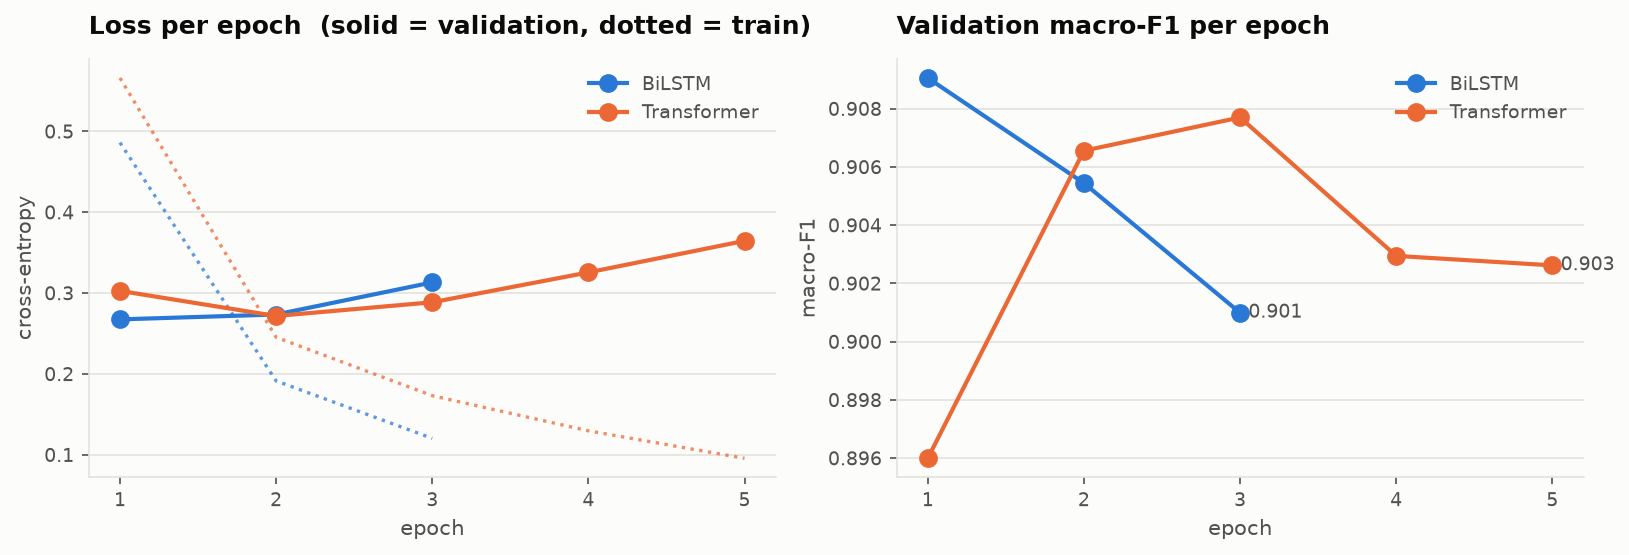
\includegraphics[width=\textwidth]{figures/fig3_learning_curves.png}
\caption[Learning curves]{Learning curves. Left: cross-entropy per epoch, solid for validation and
dotted for training. Right: validation macro-$F_1$. The divergence between training
and validation loss from epoch~2 is the overfitting referred to in the text.}
\label{fig:curves}
\end{figure}

\section{Headline results}

\begin{table}[ht]
\centering
\caption[Headline test-set results]{Headline results on the held-out test set. The accuracy
difference is 0.09 percentage points, corresponding to seven documents out of 7{,}600.}
\label{tab:headline}
\begin{tabular}{lrrrr}
\toprule
\textbf{Model} & \textbf{Accuracy} & \textbf{Macro $F_1$} & \textbf{Weighted $F_1$} & \textbf{Test loss} \\
\midrule
BiLSTM      & 0.9114 & 0.9111 & 0.9111 & 0.2797 \\
Transformer & 0.9105 & 0.9104 & 0.9104 & 0.2944 \\
\midrule
Difference  & 0.0009 & 0.0007 & 0.0007 & $-0.0147$ \\
\bottomrule
\end{tabular}
\end{table}

Both models land in the 90--92\% band anticipated by the survey of published results in
Table~\ref{tab:prior}, which is the expected range for a from-scratch model without pretraining.
The recurrent model is nominally ahead on every metric except test loss.

\keypoint{This difference must not be interpreted before it is tested.} A gap of 0.09 percentage
points on 7{,}600 documents is seven documents. Section~\ref{sec:significance} determines whether
that is distinguishable from noise. It is not.

\section{Per-class performance}

\begin{table}[ht]
\centering
\caption[Per-class results]{Per-class precision, recall and $F_1$. Support is 1{,}900
documents for every class.}
\label{tab:per_class}
\begin{tabular}{lrrrcrrr}
\toprule
 & \multicolumn{3}{c}{\textbf{BiLSTM}} & & \multicolumn{3}{c}{\textbf{Transformer}} \\
\textbf{Class} & \textbf{P} & \textbf{R} & \textbf{$F_1$} & & \textbf{P} & \textbf{R} & \textbf{$F_1$} \\
\midrule
World     & 0.9366 & 0.8789 & 0.9069 & & 0.9227 & 0.9053 & 0.9139 \\
Sports    & 0.9459 & 0.9853 & 0.9652 & & 0.9553 & 0.9674 & 0.9613 \\
Business  & 0.8850 & 0.8705 & 0.8777 & & 0.8889 & 0.8674 & 0.8780 \\
Sci/Tech  & 0.8791 & 0.9111 & 0.8948 & & 0.8754 & 0.9021 & 0.8885 \\
\midrule
Macro avg & 0.9117 & 0.9114 & 0.9111 & & 0.9106 & 0.9105 & 0.9104 \\
\bottomrule
\end{tabular}
\end{table}

\begin{figure}[ht]
\centering
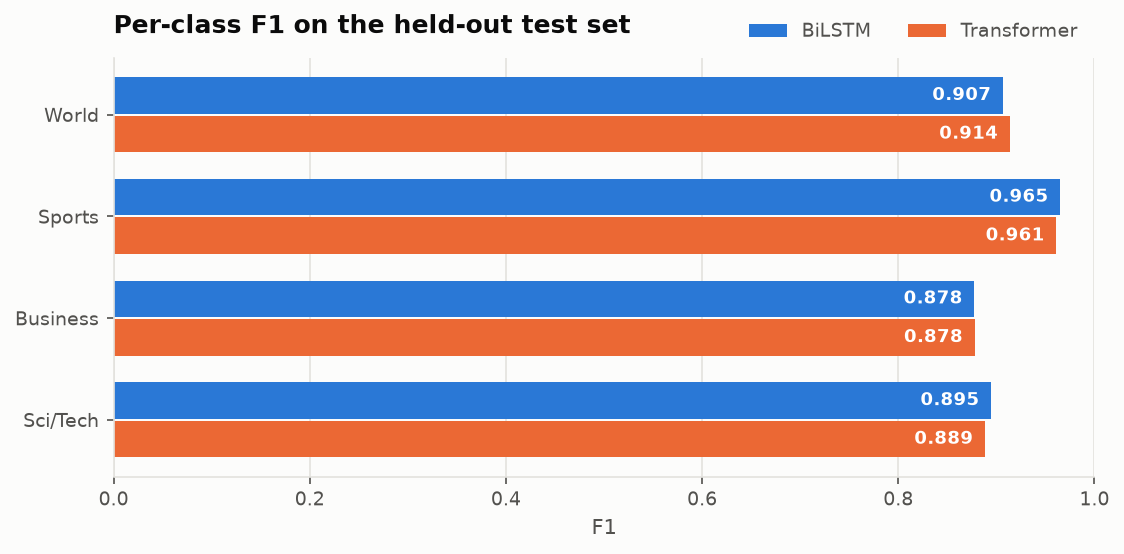
\includegraphics[width=\textwidth]{figures/fig1_per_class_f1.png}
\caption[Per-class F1 comparison]{Per-class $F_1$ for both models. The difficulty
ordering is identical: Sports is easiest for both, Business hardest for both.}
\label{fig:perclass}
\end{figure}

The striking feature of Table~\ref{tab:per_class} is not the magnitude of any difference but the
\emph{similarity of the profile}. Both models order the classes identically by difficulty:

\begin{center}
Sports ($\approx 0.96$) $\;>\;$ World ($\approx 0.91$) $\;>\;$ Sci/Tech ($\approx 0.89$) $\;>\;$ Business ($\approx 0.878$)
\end{center}

On Business the two models agree to four decimal places (0.8777 versus 0.8780). The two
architectures do not merely achieve the same aggregate accuracy; they find the same classes easy
and the same classes hard, to a degree that suggests both are limited by the same property of the
data rather than by their own representational capacity.

\section{Confusion structure}

\begin{figure}[ht]
\centering
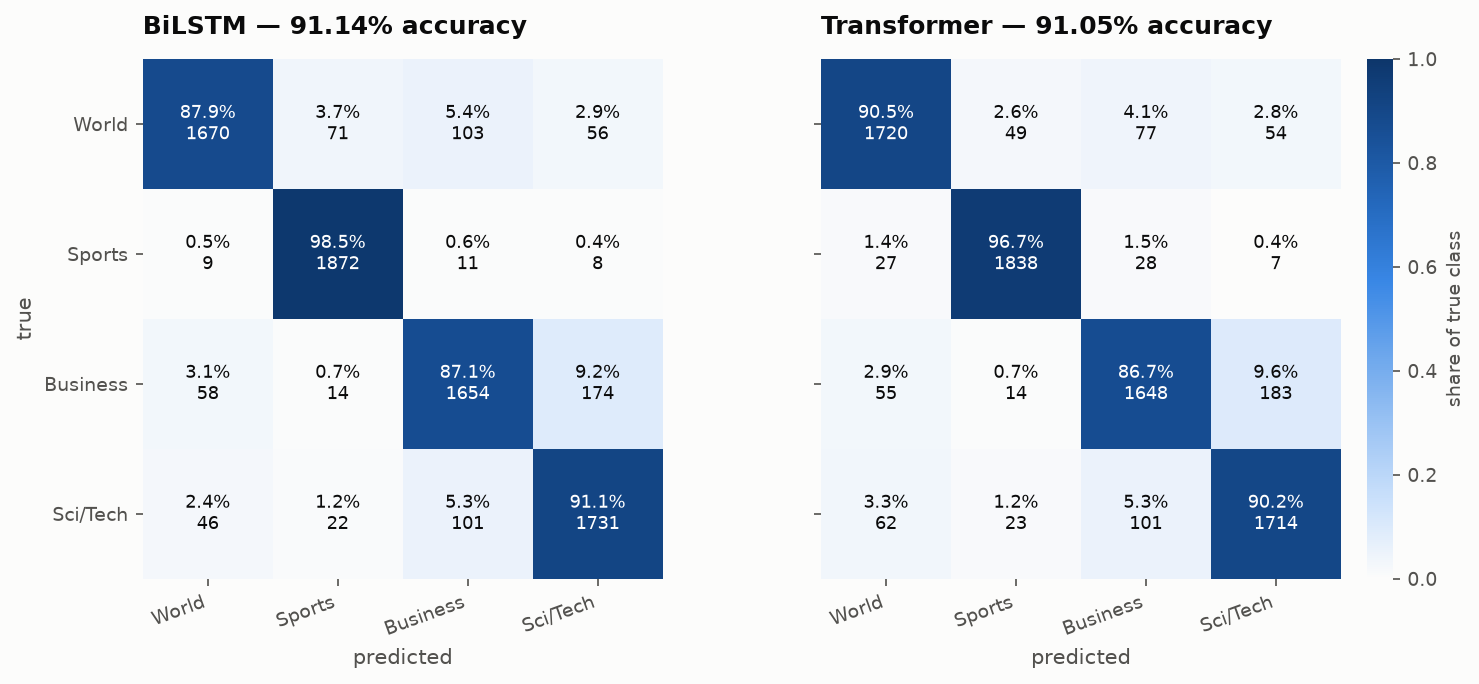
\includegraphics[width=\textwidth]{figures/fig2_confusion_matrices.png}
\caption[Confusion matrices]{Row-normalised confusion matrices on a shared colour scale. Each row
sums to 100\% of the true class. The dominant off-diagonal cell is Business predicted as Sci/Tech
for both models.}
\label{fig:confusion}
\end{figure}

\begin{table}[ht]
\centering
\caption{Largest off-diagonal confusions, as a proportion of the true class.}
\label{tab:confusions}
\begin{tabular}{llrr}
\toprule
\textbf{True} & \textbf{Predicted} & \textbf{BiLSTM} & \textbf{Transformer} \\
\midrule
Business & Sci/Tech & 9.2\% (174) & 9.6\% (183) \\
World    & Business & 5.4\% (103) & 4.1\% (77) \\
Sci/Tech & Business & 5.3\% (101) & 5.3\% (101) \\
World    & Sports   & 3.7\% (71)  & 2.6\% (49) \\
\bottomrule
\end{tabular}
\end{table}

The structure is consistent across both models. The dominant error is Business misclassified as
Sci/Tech, and its converse is the third largest. Together, the Business--Sci/Tech boundary accounts
for roughly a quarter of all errors made by either model.

Sports is nearly separable from everything else --- 98.5\% and 96.7\% recall --- which is
unsurprising given its highly distinctive vocabulary. The difficulty is concentrated entirely in
the commercial and technological categories, whose vocabularies overlap substantially.

\section{Statistical significance}
\label{sec:significance}

Applying McNemar's test as specified in Section~\ref{sec:mcnemar} to the paired predictions:

\begin{table}[ht]
\centering
\caption[McNemar contingency table]{McNemar contingency table on the 7{,}600 test documents.}
\label{tab:mcnemar}
\begin{tabular}{lrr}
\toprule
 & \textbf{BiLSTM correct} & \textbf{BiLSTM wrong} \\
\midrule
\textbf{Transformer correct} & 6{,}740 & 180 \\
\textbf{Transformer wrong}   & 187     & 493 \\
\bottomrule
\end{tabular}
\end{table}

The models agree on $6{,}740 + 493 = 7{,}233$ documents, or \textbf{94.78\%} of the test set. The
discordant set contains 367 documents: 187 answered correctly only by the recurrent model and 180
only by the Transformer.

Under the null hypothesis of equal error rates, the number falling to either model follows
$\operatorname{Binomial}(367, 0.5)$. The exact binomial test gives
\begin{equation}
p = 0.754 .
\end{equation}

\keypoint{The difference is not statistically significant at $\alpha = 0.05$.} A split of 187
against 180 is as close to an even division as a test set of this size can resolve. The correct
conclusion is that \textbf{the two architectures are indistinguishable in accuracy on this task} --
not that the recurrent model is marginally superior.

This is the central result of the study, and it would have been inaccessible from the headline
accuracy figures alone. A 0.09 percentage point gap presented without a significance test invites
exactly the over-interpretation that the test forecloses.

\section{Computational cost}
\label{sec:cost}

\begin{table}[ht]
\centering
\caption[Computational cost]{Computational cost on the CPU-only environment of
Table~\ref{tab:environment}.}
\label{tab:cost}
\begin{tabular}{lrr}
\toprule
\textbf{Measure} & \textbf{BiLSTM} & \textbf{Transformer} \\
\midrule
Non-embedding parameters  & 265{,}220 & 265{,}732 \\
Seconds per epoch         & 41.2 & 68.6 \\
Total training time (s)   & 126  & 353 \\
Inference (ms per 1{,}000 documents) & 138 & 335 \\
Test accuracy             & 0.9114 & 0.9105 \\
\bottomrule
\end{tabular}
\end{table}

At matched capacity and matched accuracy, the recurrent model trains \textbf{1.67 times faster per
epoch} and performs inference \textbf{2.43 times faster}.

\keypoint{This is the opposite of the expected result, and it requires careful interpretation
rather than explanation away.}

The standard argument, formalised in Table~\ref{tab:complexity}, is that recurrence requires $O(n)$
strictly sequential steps whereas self-attention requires $O(1)$, so attention should be faster in
wall-clock terms. That argument is correct, but it is an argument about \emph{parallelisability},
and it is conditional on two things that do not hold here.

First, \textbf{parallel hardware}. The advantage of $O(1)$ sequential depth is realised only when
there are parallel resources to exploit. On six CPU threads there is very little parallelism
available, so the Transformer cannot convert its structural advantage into elapsed time.

Second, \textbf{the relationship between $n$ and $d$}. Per-layer arithmetic is $O(n d^2)$ for
recurrence and $O(n^2 d)$ for self-attention. Self-attention performs less total arithmetic only
when $n < d$. Here $n = 64$ and $d = 128$, so the two are of the same order and neither dominates.
The Transformer performs more total floating-point work per document --- two encoder blocks of
four-head attention over all 64 positions, each with a 256-wide feed-forward sublayer --- while the
recurrent model performs less work spread over 64 sequential dispatches.

When neither parallelism nor arithmetic favours attention, the constant factors decide, and here
they favour recurrence.

\keypoint{What this result does and does not license.} It does not license the claim that recurrent
networks are faster than Transformers. It licenses the narrower and more useful claim that
\emph{at short sequence lengths on sequential hardware, the Transformer's architectural advantage
does not materialise in wall-clock terms}. The recurrent model's disadvantage grows linearly with
sequence length, and on parallel hardware the ordering would be expected to reverse. This is a
finding about regime, not about architecture, and it is actionable precisely for that reason.

\section{Qualitative error analysis}

\subsection{Documents both models misclassify}

Of the 7{,}600 test documents, 493 are misclassified by both models. Table~\ref{tab:both_wrong}
gives a representative sample.

\begin{table}[ht]
\centering
\caption[Documents misclassified by both models]{Representative documents misclassified by both
models. In each case the predicted label is defensible.}
\label{tab:both_wrong}
\begin{tabular}{llp{7.3cm}}
\toprule
\textbf{True} & \textbf{Both predicted} & \textbf{Document (truncated)} \\
\midrule
Sci/Tech & World    & U.N. Urges Funds to Curb African Locusts --- with swarms threatening crops in a number of African countries \ldots \\
World    & Sports   & Argentina Basketball Coach Magnano Quits --- Ruben Magnano, who coached Argentina to the Olympic gold medal \ldots \\
Business & Sci/Tech & SBC links e-mail, voice messages, fax --- SBC announced a new service that integrates voice messages, faxes \ldots \\
Business & World    & Nepal blockade `blow to tourism' --- Nepal tour operators say tourists cancelled millions of dollars of bookings \ldots \\
Sci/Tech & World    & Singapore Telecom ties up with Malaysia's TIME dotcom --- SingTel said it has \ldots \\
\bottomrule
\end{tabular}
\end{table}

In every case the prediction is defensible. A story about United Nations funding to control locust
swarms is an international affairs story \emph{and} an agricultural science story. A telecoms
merger is a business story \emph{and} a technology story. These are not model failures in any
useful sense; they are documents whose single gold label is one of several admissible choices.

This is the practical upper bound on achievable accuracy for the task, and it explains why the
published results in Table~\ref{tab:prior} compress into such a narrow band.

\subsection{Documents on which the models disagree}

\begin{table}[ht]
\centering
\caption[Documents on which the models disagree]{Documents where the two models differ. Several
turn on a single lexical cue.}
\label{tab:disagree}
\begin{tabular}{lllp{5.4cm}}
\toprule
\textbf{True} & \textbf{BiLSTM} & \textbf{Transf.} & \textbf{Document (truncated)} \\
\midrule
Sports   & Sports   & Business & Cape Town F1 bid --- plan to build a multi-million-dollar race track \ldots \\
World    & Business & World    & ConocoPhillips boosts LUKoil stake to 10 percent \ldots \\
Business & Sports   & Business & Banks seek court ruling over F1 --- three banks go to the High Court in London \ldots \\
Sports   & Sports   & World    & New Namath Book Is Fact, Not Fiction --- if you read the recent excerpt in Sports Illustrated \ldots \\
World    & World    & Business & Australia: Wallets trump war --- a majority oppose the Iraq war, but were more concerned \ldots \\
\bottomrule
\end{tabular}
\end{table}

The disagreements are instructive. Several documents contain strong lexical evidence for two
classes simultaneously --- \emph{Formula One} alongside \emph{multi-million-dollar}, or
\emph{banks} and \emph{High Court} alongside \emph{F1} --- and the two models resolve the conflict
differently. Notably, neither model is systematically correct in these cases: the first and third
examples show the models trading places on the same underlying ambiguity.

This is consistent with the statistical finding of Section~\ref{sec:significance}. The disagreements
are not evidence of a systematic difference in capability; they are what one would expect from two
comparably-capable models resolving genuinely ambiguous cases with different random tie-breaking.

\chapter{Discussion}
\label{ch:discussion}

\section{Answering the research question}

The research question was: \emph{how do recurrent networks and Transformers compare at classifying
short news texts?} The evidence of Chapter~\ref{ch:results} supports a four-part answer.

\subsection{They are indistinguishable in accuracy}

The measured difference is 0.09 percentage points. McNemar's exact test on the paired predictions
gives $p = 0.754$, the models agree on 94.78\% of test documents, and the discordant set splits 187
to 180. There is no basis in this evidence for preferring either architecture on accuracy grounds.

This is a negative result, and it is reported as the principal finding rather than buried. Negative
results of this kind are underreported in the literature, with the consequence that accuracy
differences well inside the noise floor are routinely presented as architectural improvements. The
discipline of applying a paired significance test is what converts an apparent 0.09-point win into
the correct conclusion of equivalence.

\subsection{The explanation is document length}

The equivalence is not a coincidence, and it is not evidence that self-attention is overrated in
general. It follows from a specific property of the data.

Self-attention's structural advantage, established in Table~\ref{tab:complexity}, is a maximum path
length of $O(1)$ between any two positions, against $O(n)$ for recurrence. This is an advantage in
modelling \emph{long-range} dependency.

The median AG News document is 39 tokens long. In a 39-token document there are essentially no
long-range dependencies to model. The furthest two tokens can be is a few dozen positions, which a
bidirectional LSTM traverses without difficulty --- this is precisely the regime the gating
mechanism of Section~\ref{sec:vanishing} was designed to handle, and it is two orders of magnitude
short of where the gating mechanism begins to fail.

Furthermore, the signal in topic classification is overwhelmingly lexical. The presence of
\emph{coach}, \emph{Olympic} and \emph{medal} identifies a sports story regardless of their
arrangement. This observation is corroborated independently by the literature: FastText, which
averages word vectors and models no order whatsoever, reaches approximately 92.5\% on this
benchmark (Table~\ref{tab:prior}) --- at or above both models in this study. If a bag-of-embeddings
model is competitive, then the marginal value of \emph{any} sequence modelling on this task is
small, and the marginal value of one sequence model over another is smaller still.

\keypoint{The general form of the argument.} An architecture's advantage can only be realised on a
task that exercises the property the architecture is good at. Transformers are superior at modelling
long-range dependency; AG News contains almost none; therefore the two architectures perform
equivalently. This is not a limitation of the Transformer but a statement about the task.

\subsection{They fail in the same way}

The equivalence runs deeper than aggregate accuracy. The two models share:

\begin{itemize}
\item an identical per-class difficulty ordering (Sports, World, Sci/Tech, Business),
\item near-identical per-class $F_1$, agreeing to four decimal places on Business,
\item the same dominant confusion, Business predicted as Sci/Tech, at 9.2\% and 9.6\%,
\item agreement on 94.78\% of individual test predictions.
\end{itemize}

Two models with materially different inductive biases would be expected to differ somewhere in this
profile even at equal overall accuracy. That they do not indicates both are limited by the same
external factor. The error analysis of Chapter~\ref{ch:results} identifies that factor: documents
whose gold label is one of several admissible choices. A story about a semiconductor firm's
quarterly earnings is legitimately Business and legitimately Sci/Tech; the corpus assigns one
label, and no model can recover the other.

This is an irreducible component of the error, a property of the annotation rather than of either
model, and it caps what any architecture can achieve on this benchmark.

\subsection{Cost is where they differ, and the finding inverts expectation}

At matched accuracy and matched capacity, the recurrent model trained 1.67 times faster per epoch
and performed inference 2.43 times faster.

Section~\ref{sec:cost} analyses why. The summary is that the Transformer's advantage is
\emph{asymptotic} --- it concerns parallelisability and the growth of sequential depth with
sequence length --- and that neither condition for realising it holds in this experiment. There is
negligible hardware parallelism to exploit on six CPU threads, and at $n = 64$, $d = 128$ the
$O(n d^2)$ and $O(n^2 d)$ arithmetic costs are of the same order, so self-attention does not even
win on operation count.

The honest framing is that this is a result about a \emph{regime}, not about the architectures in
the abstract. Two predictions follow, and both are testable: the ordering should reverse on
parallel hardware, and the recurrent model's relative cost should grow linearly with sequence
length.

\section{Comparison with published results}

Both models fall within the 90--92\% band that Table~\ref{tab:prior} identifies for non-pretrained
approaches on AG News. The study therefore reproduces the expected performance level, which
provides weak corroboration that the pipeline as a whole is sound.

The roughly three-point gap to fine-tuned BERT is instructive and is worth stating plainly, since
it is frequently misattributed. That gap is \textbf{not} evidence that self-attention is a superior
architecture. It is evidence that representations learned from billions of words of unlabelled text
are superior to representations learned from 54{,}000 labelled headlines. The present study
isolates architecture by holding pretraining constant at zero for both models, and under that
control the architectural difference vanishes entirely.

This distinction matters practically. An engineer choosing between a BiLSTM and a Transformer
encoder for a short-text classification task, both trained from scratch, should not expect the
accuracy gain reported for BERT to transfer to that choice.

\section{Implications}

\keypoint{For practice.} On short-text topic classification at this scale, selecting between these
two architectures on expected accuracy is not supported by evidence. The decision should be made on
engineering grounds --- latency, memory, deployment constraints, tooling --- and those costs should
be \emph{measured on the target hardware and sequence length} rather than assumed from asymptotic
arguments. The cost finding here is a concrete demonstration that the assumed ordering can be
wrong.

\keypoint{For evaluation methodology.} Reporting a sub-point accuracy difference without a paired
significance test is not sound practice. The test applied here cost a few lines of code and
reversed the qualitative conclusion, from ``the BiLSTM is slightly better'' to ``the models are
indistinguishable''.

\keypoint{For from-scratch implementation.} The verification suite of
Chapter~\ref{ch:verification} is a transferable methodology. The key insight is that numerical code
of this kind fails silently, so verification must consist of equivalence against independent
implementations and assertion of mathematical invariants, not merely the observation that training
loss decreases.

\section{Threats to validity}
\label{sec:threats}

\subsection{Internal validity}

\keypoint{Single seed.} This is the most serious limitation. Each architecture was trained once,
with one seed. The observed 0.09-point difference is well within typical run-to-run variance for
models of this size, which is precisely why Section~\ref{sec:significance} reports a significance
test rather than a winner. The conclusion supported is ``indistinguishable''; a claim that one
architecture is genuinely superior --- in either direction --- would require multiple seeds and a
confidence interval. The study does not make such a claim.

\keypoint{Learning rates differ.} Defended in Chapter~\ref{ch:method}: the controlled quantity is
the compute budget, and both rates were selected on validation data. Residual risk remains that a
more exhaustive search would favour one architecture.

\keypoint{Both models overfit quickly.} The recurrent model peaked after one epoch. Stronger
regularisation might alter the comparison, although both models were selected at their respective
optima by the early-stopping criterion.

\subsection{External validity}

\keypoint{One corpus, one length regime.} All conclusions concern English short news text with a
median length of 39 tokens. The central finding is explicitly \emph{conditional} on that length,
and the report predicts it would not hold for longer documents.

\keypoint{No pretraining.} The findings concern architectures trained from scratch and do not
transfer to the pretrained setting.

\keypoint{CPU-only timing.} Every figure in Section~\ref{sec:cost} is specific to the hardware of
Table~\ref{tab:environment} and would be expected to change on a GPU.

\keypoint{Reduced training set.} 60{,}000 of 120{,}000 available records were used, per the brief.
The more parameter-hungry Transformer might benefit disproportionately from the full corpus.

\subsection{Construct validity}

\keypoint{Truncation.} \code{MAX\us{}LEN} of 64 truncates 3.06\% of training documents. This affects
both models identically and is unlikely to bias the comparison.

\keypoint{Simple tokenisation.} A subword tokeniser would likely raise both models' absolute
accuracy. It was omitted to keep the input identical across architectures, at a known cost in
absolute performance.

\keypoint{Label noise.} As the error analysis shows, a meaningful proportion of test documents
admit more than one defensible label. This places a ceiling on measurable accuracy and compresses
the range within which architectures can be distinguished --- which, it should be acknowledged,
makes an equivalence finding easier to obtain. A task with cleaner labels and longer documents
would be a more discriminating test.

\chapter{Conclusion and Future Work}
\label{ch:conclusion}

\section{Summary}

This report has presented a controlled comparison of a bidirectional LSTM and a Transformer encoder
on four-class news topic classification, with both architectures implemented from first principles
and verified numerically before use.

The experimental design held data, preprocessing, capacity and training budget fixed, so that
architecture was the only free variable. Non-embedding parameter counts were matched to within
0.19\%. Nine verification checks confirmed the hand-written layers against reference
implementations and mathematical invariants, all passing, before any result was generated.

\section{Findings}

\keypoint{Finding 1 --- the architectures are statistically indistinguishable in accuracy.}
91.14\% against 91.05\%, with McNemar's exact test returning $p = 0.754$ and the models agreeing on
94.78\% of test documents. The observed difference of seven documents out of 7{,}600 cannot be
separated from sampling noise.

\keypoint{Finding 2 --- document length explains the equivalence.} The median document is 39
tokens. Self-attention's structural advantage is constant-path-length access between distant
positions, and a 39-token document contains almost no such distance. The finding is corroborated by
the literature: FastText, which models no word order at all, is competitive on this benchmark.

\keypoint{Finding 3 --- both models fail identically.} Identical per-class difficulty ordering,
per-class $F_1$ agreeing to four decimal places on the hardest class, and a shared
dominant confusion between Business and Sci/Tech accounting for roughly a quarter of all errors.
Qualitative inspection shows these are documents with more than one defensible label --- a property
of the annotation, not of either model.

\keypoint{Finding 4 --- the cost comparison inverts the expected ordering.} The recurrent model
trained 1.67 times faster per epoch and performed inference 2.43 times faster. The report attributes
this to the absence of the two conditions required for self-attention's asymptotic advantage to
materialise: hardware parallelism, and a sequence length exceeding the model dimension.

\section{Contributions revisited}

The study contributes a fully transparent implementation of both architectures; a transferable
verification methodology for hand-written numerical layers; a genuinely controlled architectural
comparison; a statistically disciplined negative result; and a cost measurement that contradicts
the assumed ordering, together with an analysis of the conditions under which that ordering holds.

\section{Future work}

\keypoint{Multiple seeds.} The single most valuable extension. Training both architectures across
ten or more seeds would yield confidence intervals and would convert the present
``indistinguishable'' into a quantified bound on the maximum plausible difference. This is the
direct remedy for the principal threat to validity identified in Section~\ref{sec:threats}.

\keypoint{Sequence length sweep.} The central claim is that the equivalence is conditional on
document length. This is directly testable: evaluating both architectures on corpora of
systematically increasing document length should show the Transformer's advantage emerging as a
function of length. A positive result would confirm the explanatory mechanism; a negative result
would refute it.

\keypoint{Parallel hardware.} Repeating the cost measurement on a GPU would test the prediction
that the observed timing ordering reverses when parallel resources are available.

\keypoint{Ablation studies.} Controlled variation of bidirectionality, head count, encoder depth
and pooling strategy would separate the contribution of each design decision from the architectural
family.

\keypoint{Attention interpretability.} Visualising the learned attention distributions would
indicate whether the encoder learns locally-concentrated patterns --- which would be further
evidence for the document-length explanation --- or distributes attention broadly.

\keypoint{Pretraining.} Comparing a pretrained Transformer against a pretrained recurrent model on
identical corpora would isolate the architectural contribution in the pretrained setting, where
most practical systems now operate.

\section{Closing remarks}

The most useful result of this study is a negative one, obtained only because a significance test
was applied to a difference that looked, on its face, like a result. The second most useful is a
cost measurement that contradicted the expectation stated at the outset of the work and was
reported as measured rather than adjusted toward the textbook claim.

Both outcomes point the same way. An architecture's advantages are conditional on the task
exercising the properties that architecture provides, and on the hardware being able to realise
them. Neither condition should be assumed; both can be measured.

\begin{thebibliography}{99}
\bibitem{ba2016} J.~L. Ba, J.~R. Kiros, and G.~E. Hinton, ``Layer normalization,'' \textit{arXiv preprint arXiv:1607.06450}, 2016.
\bibitem{bahdanau2015} D.~Bahdanau, K.~Cho, and Y.~Bengio, ``Neural machine translation by jointly learning to align and translate,'' in \textit{Proc. ICLR}, 2015.
\bibitem{bengio1994} Y.~Bengio, P.~Simard, and P.~Frasconi, ``Learning long-term dependencies with gradient descent is difficult,'' \textit{IEEE Trans. Neural Networks}, vol.~5, no.~2, pp.~157--166, 1994.
\bibitem{cho2014} K.~Cho et~al., ``Learning phrase representations using RNN encoder--decoder for statistical machine translation,'' in \textit{Proc. EMNLP}, 2014.
\bibitem{devlin2019} J.~Devlin, M.-W. Chang, K.~Lee, and K.~Toutanova, ``BERT: Pre-training of deep bidirectional transformers for language understanding,'' in \textit{Proc. NAACL-HLT}, 2019.
\bibitem{gers2000} F.~A. Gers, J.~Schmidhuber, and F.~Cummins, ``Learning to forget: Continual prediction with LSTM,'' \textit{Neural Computation}, vol.~12, no.~10, pp.~2451--2471, 2000.
\bibitem{hochreiter1997} S.~Hochreiter and J.~Schmidhuber, ``Long short-term memory,'' \textit{Neural Computation}, vol.~9, no.~8, pp.~1735--1780, 1997.
\bibitem{joachims1998} T.~Joachims, ``Text categorization with support vector machines,'' in \textit{Proc. ECML}, 1998.
\bibitem{joulin2017} A.~Joulin, E.~Grave, P.~Bojanowski, and T.~Mikolov, ``Bag of tricks for efficient text classification,'' in \textit{Proc. EACL}, 2017.
\bibitem{kingma2015} D.~P. Kingma and J.~Ba, ``Adam: A method for stochastic optimization,'' in \textit{Proc. ICLR}, 2015.
\bibitem{liu2019} Y.~Liu et~al., ``RoBERTa: A robustly optimized BERT pretraining approach,'' \textit{arXiv preprint arXiv:1907.11692}, 2019.
\bibitem{loshchilov2019} I.~Loshchilov and F.~Hutter, ``Decoupled weight decay regularization,'' in \textit{Proc. ICLR}, 2019.
\bibitem{luong2015} M.-T. Luong, H.~Pham, and C.~D. Manning, ``Effective approaches to attention-based neural machine translation,'' in \textit{Proc. EMNLP}, 2015.
\bibitem{mcnemar1947} Q.~McNemar, ``Note on the sampling error of the difference between correlated proportions or percentages,'' \textit{Psychometrika}, vol.~12, no.~2, pp.~153--157, 1947.
\bibitem{mdpi2024} ``A study on text classification in the age of large language models,'' \textit{Machine Learning and Knowledge Extraction}, MDPI, 2024.
\bibitem{mikolov2013} T.~Mikolov, K.~Chen, G.~Corrado, and J.~Dean, ``Efficient estimation of word representations in vector space,'' in \textit{Proc. ICLR Workshop}, 2013.
\bibitem{pascanu2013} R.~Pascanu, T.~Mikolov, and Y.~Bengio, ``On the difficulty of training recurrent neural networks,'' in \textit{Proc. ICML}, 2013.
\bibitem{paszke2019} A.~Paszke et~al., ``PyTorch: An imperative style, high-performance deep learning library,'' in \textit{Proc. NeurIPS}, 2019.
\bibitem{pennington2014} J.~Pennington, R.~Socher, and C.~D. Manning, ``GloVe: Global vectors for word representation,'' in \textit{Proc. EMNLP}, 2014.
\bibitem{schuster1997} M.~Schuster and K.~K. Paliwal, ``Bidirectional recurrent neural networks,'' \textit{IEEE Trans. Signal Processing}, vol.~45, no.~11, pp.~2673--2681, 1997.
\bibitem{srivastava2014} N.~Srivastava et~al., ``Dropout: A simple way to prevent neural networks from overfitting,'' \textit{JMLR}, vol.~15, pp.~1929--1958, 2014.
\bibitem{vaswani2017} A.~Vaswani et~al., ``Attention is all you need,'' in \textit{Proc. NeurIPS}, 2017.
\bibitem{xiong2020} R.~Xiong et~al., ``On layer normalization in the transformer architecture,'' in \textit{Proc. ICML}, 2020.
\bibitem{zhang2015} X.~Zhang, J.~Zhao, and Y.~LeCun, ``Character-level convolutional networks for text classification,'' in \textit{Proc. NeurIPS}, 2015.
\end{thebibliography}
\addcontentsline{toc}{chapter}{References}

\appendix

\chapter{Reproduction}
\label{app:repro}

Every number in this report is produced by executing the notebook
\code{ag\us{}news\us{}rnn\us{}vs\us{}transformer.ipynb} end to end. The repository is at
\url{https://github.com/Ashwin-3cS/transformer-t1}.

\section{Environment}

{\small
\begin{verbatim}
uv venv .venv --python 3.14
uv pip install --python .venv/bin/python torch \
    --index-url https://download.pytorch.org/whl/cpu
uv pip install --python .venv/bin/python -r requirements.txt
.venv/bin/python -m ipykernel install --user --name laksh-agnews \
    --display-name "AG News (scratch models)"
\end{verbatim}}

\section{Data access}

The corpus is downloaded through the Kaggle API on first run and cached in \code{data/agnews/}.
The newer Kaggle token format is used:

{\small
\begin{verbatim}
mkdir -p ~/.kaggle
echo KGAT_xxxxxxxx > ~/.kaggle/access_token
chmod 600 ~/.kaggle/access_token
\end{verbatim}}

A legacy \code{~/.kaggle/kaggle.json} credential file is also accepted. If neither is present the
notebook raises an explanatory error rather than failing with an opaque HTTP status.

\section{Execution}

{\small
\begin{verbatim}
MPLBACKEND=Agg .venv/bin/jupyter nbconvert --to notebook --execute --inplace \
    --ExecutePreprocessor.timeout=7200 ag_news_rnn_vs_transformer.ipynb
\end{verbatim}}

Total runtime on the reference hardware is approximately nine minutes: 126\,s of recurrent model
training, 353\,s of Transformer training, plus data acquisition, encoding and evaluation.

Setting \code{SMOKE\us{}TEST = True} in the configuration cell reduces the experiment to 2{,}000
records and one epoch, allowing the whole notebook to execute in about a minute. This is
recommended before committing to a full run.

\section{Outputs}

Execution writes to \code{artifacts/}: \code{metrics.json} containing every reported figure in
machine-readable form, both model checkpoints, and the four figures reproduced in this report.

\section{Determinism}

All random number generators are seeded at 42. The experiment was executed twice during
preparation of this report. Accuracy, macro-$F_1$, weighted $F_1$,
per-class $F_1$, parameter counts and the complete McNemar contingency table were
identical between runs. Only wall-clock timings varied, as expected.

\chapter{Complete Classification Reports}
\label{app:reports}

Generated on the 7{,}600-document test set. Support is 1{,}900 for every class.

\section{Model A --- bidirectional LSTM}

{\small
\begin{verbatim}
              precision    recall  f1-score   support

       World     0.9366    0.8789    0.9069      1900
      Sports     0.9459    0.9853    0.9652      1900
    Business     0.8850    0.8705    0.8777      1900
    Sci/Tech     0.8791    0.9111    0.8948      1900

    accuracy                         0.9114      7600
   macro avg     0.9117    0.9114    0.9111      7600
weighted avg     0.9117    0.9114    0.9111      7600
\end{verbatim}}

\section{Model B --- Transformer encoder}

{\small
\begin{verbatim}
              precision    recall  f1-score   support

       World     0.9227    0.9053    0.9139      1900
      Sports     0.9553    0.9674    0.9613      1900
    Business     0.8889    0.8674    0.8780      1900
    Sci/Tech     0.8754    0.9021    0.8885      1900

    accuracy                         0.9105      7600
   macro avg     0.9106    0.9105    0.9104      7600
weighted avg     0.9106    0.9105    0.9104      7600
\end{verbatim}}

\section{Confusion matrices, absolute counts}

\begin{table}[ht]
\centering
\caption{Confusion matrix, bidirectional LSTM. Rows are true classes.}
\begin{tabular}{lrrrr}
\toprule
 & \textbf{World} & \textbf{Sports} & \textbf{Business} & \textbf{Sci/Tech} \\
\midrule
World    & 1670 & 71   & 103  & 56 \\
Sports   & 9    & 1872 & 11   & 8 \\
Business & 58   & 14   & 1654 & 174 \\
Sci/Tech & 46   & 22   & 101  & 1731 \\
\bottomrule
\end{tabular}
\end{table}

\begin{table}[ht]
\centering
\caption{Confusion matrix, Transformer encoder. Rows are true classes.}
\begin{tabular}{lrrrr}
\toprule
 & \textbf{World} & \textbf{Sports} & \textbf{Business} & \textbf{Sci/Tech} \\
\midrule
World    & 1720 & 49   & 77   & 54 \\
Sports   & 27   & 1838 & 28   & 7 \\
Business & 55   & 14   & 1648 & 183 \\
Sci/Tech & 62   & 23   & 101  & 1714 \\
\bottomrule
\end{tabular}
\end{table}

\chapter{Source Listings}
\label{app:source}

Complete listings of the from-scratch components. The training harness, preprocessing pipeline and
evaluation code are in the notebook and are omitted here for brevity.

\section{Transformer encoder, complete}

{\small
\begin{verbatim}
def sinusoidal_positional_encoding(max_len, d_model):
    position = torch.arange(max_len, dtype=torch.float32).unsqueeze(1)
    even_i   = torch.arange(0, d_model, 2, dtype=torch.float32)
    div_term = torch.exp(-math.log(10000.0) * even_i / d_model)
    pe = torch.zeros(max_len, d_model)
    pe[:, 0::2] = torch.sin(position * div_term)
    pe[:, 1::2] = torch.cos(position * div_term)[:, : pe[:, 1::2].shape[1]]
    return pe


class LayerNormScratch(nn.Module):
    def __init__(self, d_model, eps=1e-5):
        super().__init__()
        self.gamma = nn.Parameter(torch.ones(d_model))
        self.beta  = nn.Parameter(torch.zeros(d_model))
        self.eps = eps

    def forward(self, x):
        mu  = x.mean(dim=-1, keepdim=True)
        var = x.var(dim=-1, keepdim=True, unbiased=False)
        return self.gamma * (x - mu) / torch.sqrt(var + self.eps) + self.beta


class MultiHeadSelfAttentionScratch(nn.Module):
    def __init__(self, d_model, n_heads, dropout=0.0):
        super().__init__()
        assert d_model % n_heads == 0
        self.n_heads, self.d_k = n_heads, d_model // n_heads
        self.W_q = nn.Linear(d_model, d_model)
        self.W_k = nn.Linear(d_model, d_model)
        self.W_v = nn.Linear(d_model, d_model)
        self.W_o = nn.Linear(d_model, d_model)
        self.dropout = nn.Dropout(dropout)

    def _split_heads(self, t):
        B, T, _ = t.shape
        return t.view(B, T, self.n_heads, self.d_k).transpose(1, 2)

    def forward(self, x, key_mask=None, return_attention=False):
        B, T, _ = x.shape
        q = self._split_heads(self.W_q(x))
        k = self._split_heads(self.W_k(x))
        v = self._split_heads(self.W_v(x))

        scores = (q @ k.transpose(-2, -1)) / math.sqrt(self.d_k)
        if key_mask is not None:
            scores = scores.masked_fill(key_mask[:, None, None, :] == 0, -1e9)

        attention = torch.softmax(scores, dim=-1)
        context = self.dropout(attention) @ v
        context = context.transpose(1, 2).reshape(B, T, self.n_heads * self.d_k)
        out = self.W_o(context)
        return (out, attention) if return_attention else out


class EncoderBlockScratch(nn.Module):
    def __init__(self, d_model, n_heads, d_ff, dropout):
        super().__init__()
        self.norm1 = LayerNormScratch(d_model)
        self.attention = MultiHeadSelfAttentionScratch(d_model, n_heads, dropout)
        self.norm2 = LayerNormScratch(d_model)
        self.ff_in  = nn.Linear(d_model, d_ff)
        self.ff_out = nn.Linear(d_ff, d_model)
        self.dropout = nn.Dropout(dropout)

    def forward(self, x, key_mask=None):
        x = x + self.dropout(self.attention(self.norm1(x), key_mask))
        h = self.norm2(x)
        h = self.ff_out(self.dropout(F.gelu(self.ff_in(h))))
        return x + self.dropout(h)


class TransformerClassifier(nn.Module):
    def __init__(self, vocab_size, d_model=128, n_heads=4, n_layers=2,
                 d_ff=256, max_len=64, n_classes=4, dropout=0.1):
        super().__init__()
        self.d_model = d_model
        self.embedding = nn.Embedding(vocab_size, d_model, padding_idx=PAD_ID)
        nn.init.normal_(self.embedding.weight, mean=0.0, std=0.1)
        with torch.no_grad():
            self.embedding.weight[PAD_ID].zero_()
        self.register_buffer("pos_encoding",
                             sinusoidal_positional_encoding(max_len, d_model))
        self.dropout = nn.Dropout(dropout)
        self.blocks = nn.ModuleList(
            EncoderBlockScratch(d_model, n_heads, d_ff, dropout)
            for _ in range(n_layers))
        self.norm_final = LayerNormScratch(d_model)
        self.classifier = nn.Linear(d_model, n_classes)

    def forward(self, ids, lengths=None):
        mask = (ids != PAD_ID)
        T = ids.size(1)
        x = self.embedding(ids) * math.sqrt(self.d_model) \
            + self.pos_encoding[:T].unsqueeze(0)
        x = self.dropout(x)
        for block in self.blocks:
            x = block(x, mask)
        x = self.norm_final(x)
        m = mask.float().unsqueeze(-1)
        pooled = (x * m).sum(dim=1) / m.sum(dim=1).clamp(min=1.0)
        return self.classifier(self.dropout(pooled))
\end{verbatim}}

\section{Bidirectional LSTM classifier, complete}

{\small
\begin{verbatim}
class BiLSTMClassifier(nn.Module):
    def __init__(self, vocab_size, emb_dim=128, hidden=128,
                 n_classes=4, dropout=0.30):
        super().__init__()
        self.embedding = nn.Embedding(vocab_size, emb_dim, padding_idx=PAD_ID)
        nn.init.normal_(self.embedding.weight, mean=0.0, std=0.1)
        with torch.no_grad():
            self.embedding.weight[PAD_ID].zero_()
        self.forward_layer  = LSTMLayerScratch(emb_dim, hidden, reverse=False)
        self.backward_layer = LSTMLayerScratch(emb_dim, hidden, reverse=True)
        self.dropout = nn.Dropout(dropout)
        self.classifier = nn.Linear(4 * hidden, n_classes)

    def forward(self, ids, lengths=None):
        mask = (ids != PAD_ID).float()
        x = self.embedding(ids)
        out_f, h_f = self.forward_layer(x, mask)
        out_b, h_b = self.backward_layer(x, mask)
        seq = torch.cat([out_f, out_b], dim=-1)
        denom = mask.sum(dim=1, keepdim=True).clamp(min=1.0)
        mean_pooled = (seq * mask.unsqueeze(-1)).sum(dim=1) / denom
        features = torch.cat([mean_pooled, h_f, h_b], dim=-1)
        return self.classifier(self.dropout(features))
\end{verbatim}}

\chapter{Verification Suite Output}
\label{app:verification}

Output produced on every execution, before training begins.

{\small
\begin{verbatim}
check                                            result  detail
-------------------------------------------------------------------------------
LSTM cell matches nn.LSTM                        PASS    outputs=5.96e-08
                                                         final h=4.47e-08
LayerNorm matches F.layer_norm                   PASS    max|diff|=4.77e-07
Attention matches naive per-head reference       PASS    max|diff|=8.94e-08
Attention rows sum to 1                          PASS    max|rowsum-1|=1.79e-07
Padded keys get ~zero attention                  PASS    max mass=0.00e+00
BiLSTM: logits unchanged by extra padding        PASS    max|diff|=0.00e+00
Transformer: logits unchanged by extra padding   PASS    max|diff|=1.19e-07
BiLSTM: overfits 200 examples                    PASS    accuracy=100.0%
Transformer: overfits 200 examples               PASS    accuracy=100.0%
-------------------------------------------------------------------------------
All 9 checks passed. The hand-written layers are numerically correct.
\end{verbatim}}

\chapter{Summary of Key Figures}
\label{app:summary}

\begin{table}[ht]
\centering
\caption{All headline quantities reported in this study.}
\begin{tabular}{lrr}
\toprule
\textbf{Quantity} & \textbf{BiLSTM} & \textbf{Transformer} \\
\midrule
Test accuracy                    & 0.9114 & 0.9105 \\
Macro $F_1$         & 0.9111 & 0.9104 \\
Weighted $F_1$      & 0.9111 & 0.9104 \\
Test cross-entropy               & 0.2797 & 0.2944 \\
Best validation macro-$F_1$ & 0.9091 & 0.9077 \\
Best epoch                       & 1 & 3 \\
Epochs run                       & 3 & 5 \\
Seconds per epoch                & 41.2 & 68.6 \\
Total training time (s)          & 126 & 353 \\
Inference (ms / 1000 docs)       & 138 & 335 \\
Total parameters                 & 4{,}612{,}612 & 4{,}613{,}124 \\
Non-embedding parameters         & 265{,}220 & 265{,}732 \\
\bottomrule
\end{tabular}
\end{table}

\begin{table}[ht]
\centering
\caption{Shared experimental quantities.}
\begin{tabular}{lr}
\toprule
\textbf{Quantity} & \textbf{Value} \\
\midrule
Training records          & 54{,}000 \\
Validation records        & 6{,}000 \\
Test records              & 7{,}600 \\
Vocabulary size           & 33{,}964 \\
Maximum sequence length   & 64 \\
Median document length    & 39 tokens \\
Coverage at max length    & 96.94\% \\
Verification checks passed & 9 / 9 \\
Model agreement           & 94.78\% \\
Discordant documents      & 367 \\
McNemar $p$-value         & 0.754 \\
\bottomrule
\end{tabular}
\end{table}


\end{document}
